%!TEX  root=./LIVRO.tex

\chapter{Manual de caça}\label{manual-de-cauxe7a}

\begin{figure}[H]
\centering
\captionsetup{width=87mm}
  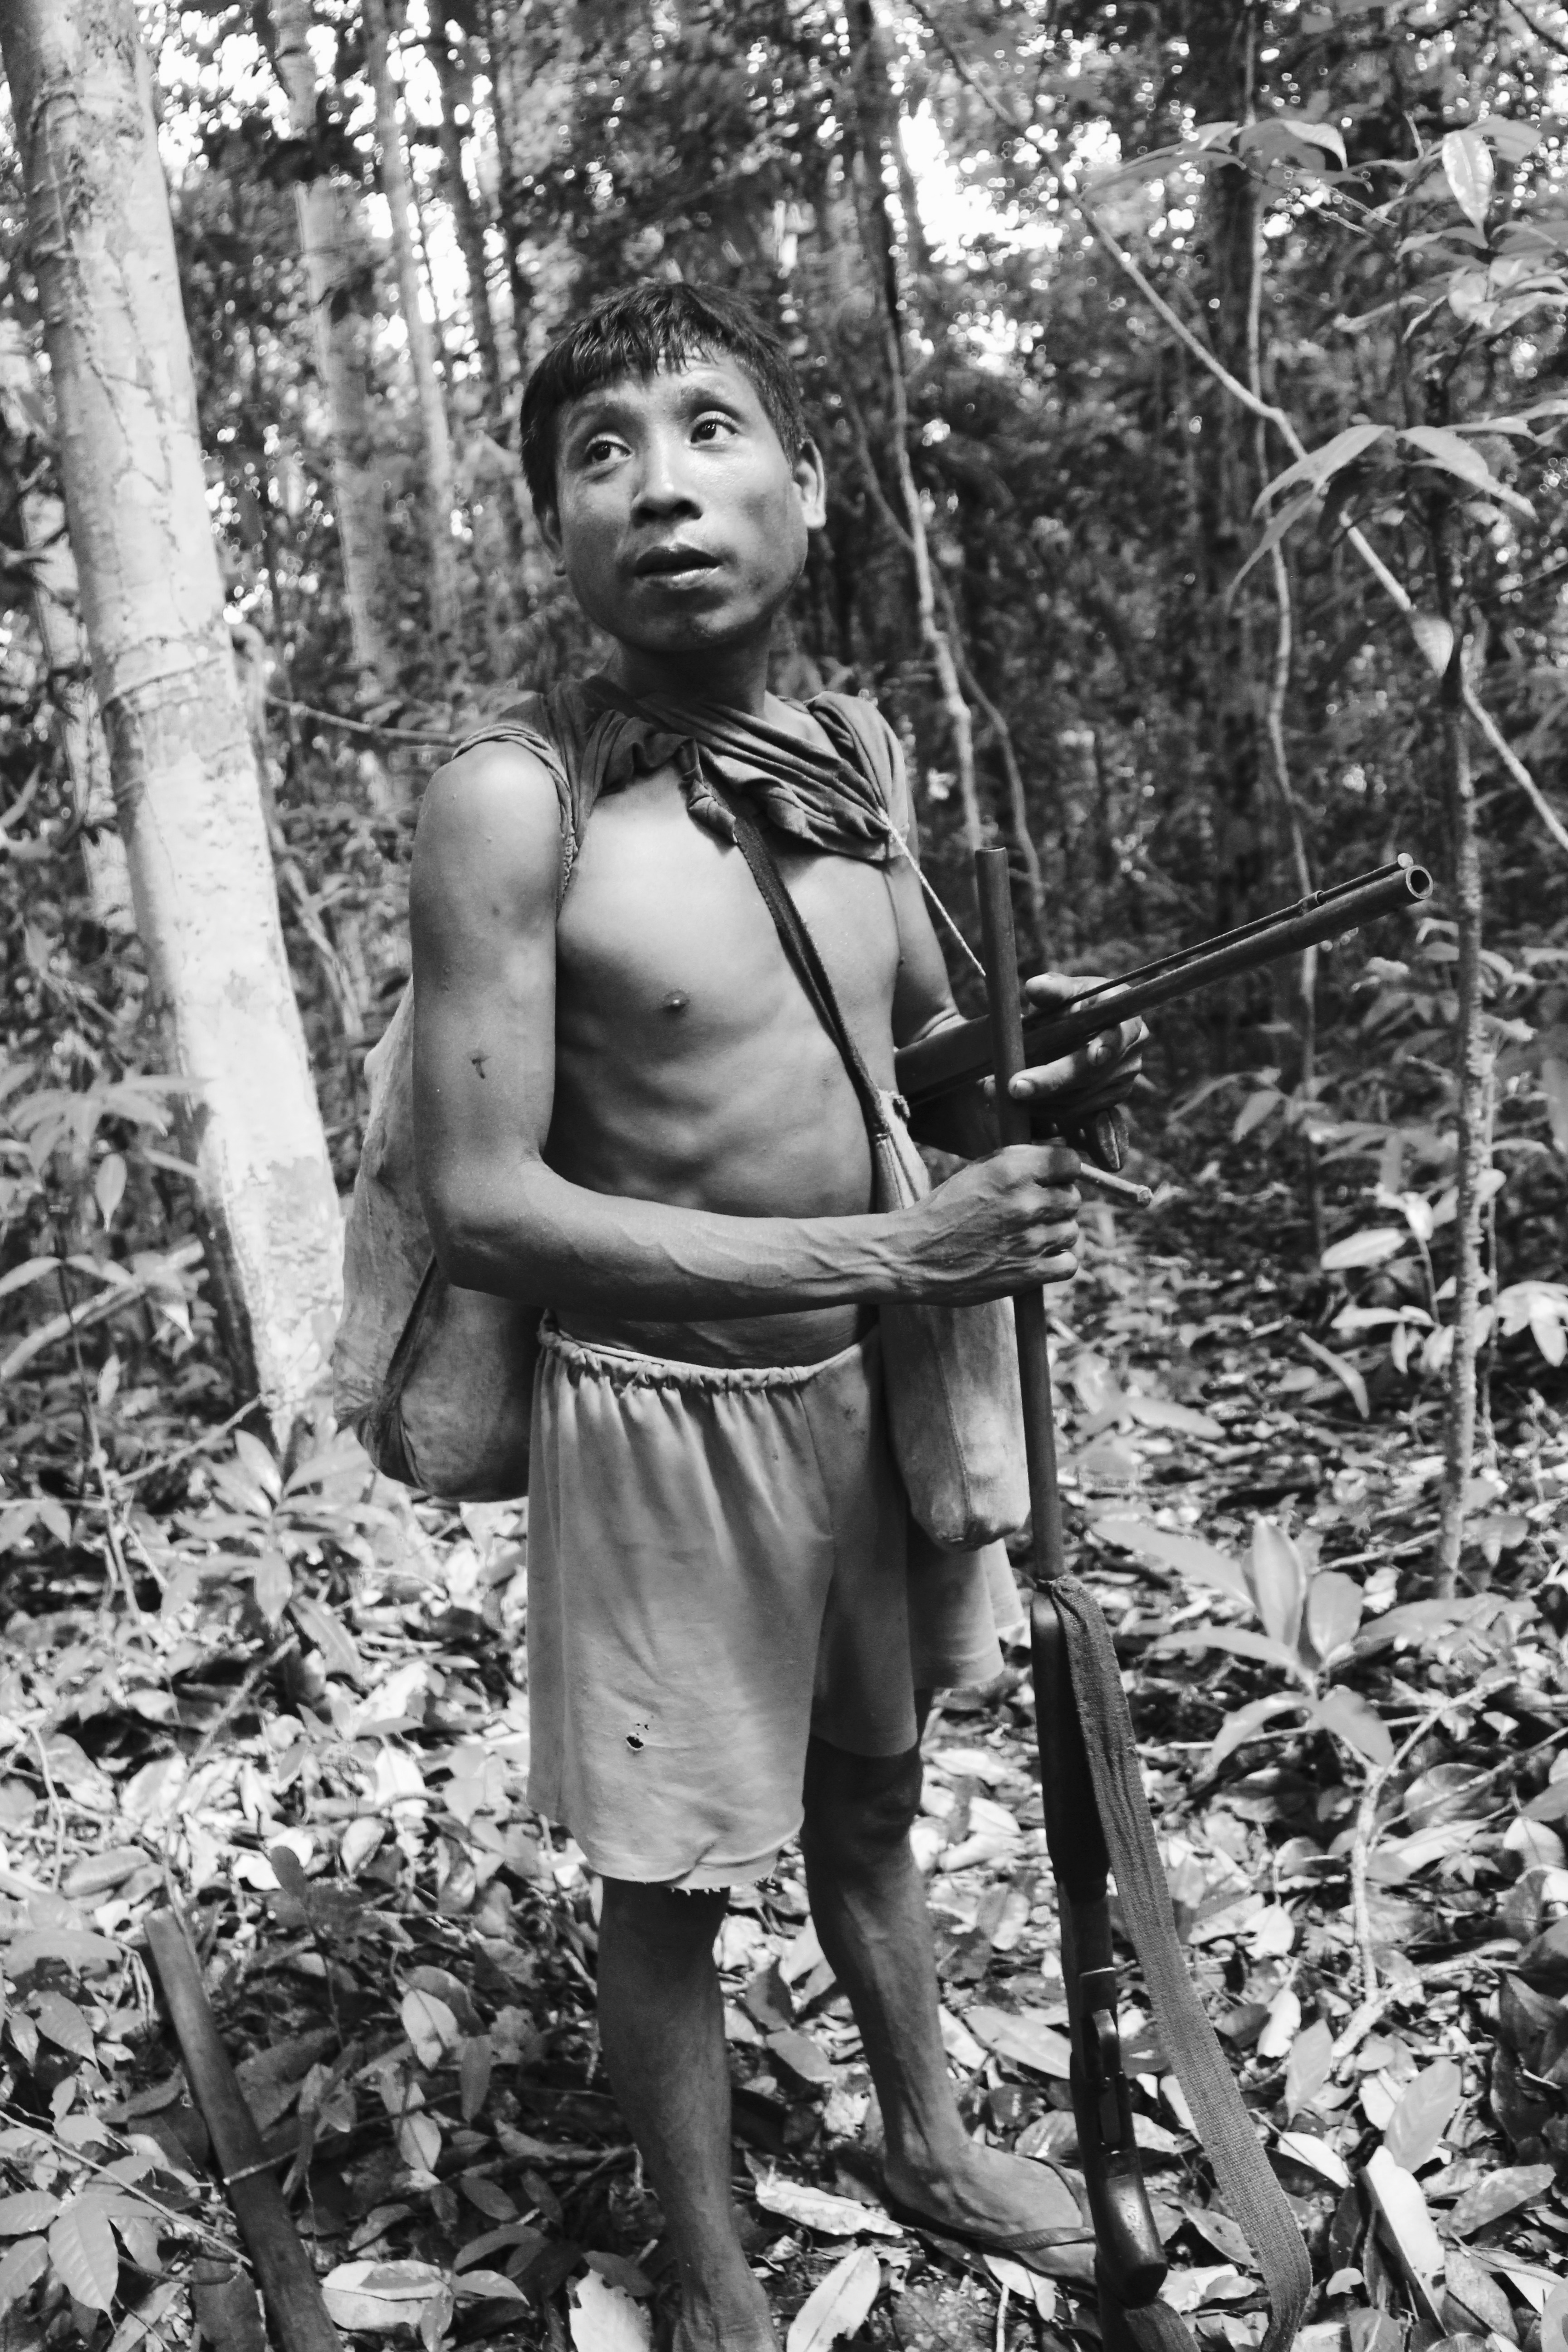
\includegraphics[width=87mm]{./imgs/IMG_1553}
\caption{Maihuxa’a durante um dia de caminhada, ajudando seu irmão a carregar uma espingarda (acampamento de caça, aldeia Awá, 2013).}
\end{figure}

\section{\emph{Waria}}\label{waria}

Os capelães são animais extraordinários. Ao menos aqueles que vivem nas
matas do Pindaré, Caru e Turiaçu. \emph{Waria}, é como os Guajá chamam
esses animais que eles caçam, criam, cuidam, comem, enfim, pelos quais
se interessam inteiramente. É no ciclo da lua cheia, sobretudo nos fins
de tarde, que o rugido do capelão pode ser ouvido por toda a floresta,
tão alto quanto as cigarras que cantam nos meses quentes. Os
bugios\footnote{Os primatas do tipo bugio compreendem diversas espécies
  do gênero \emph{Alouatta}, presentes em todo o Brasil e partes da
  América do Sul. Este animal é popularmente conhecido no Brasil como
  ``guariba'', e em boa parte da Amazônia brasileira como ``capelão''.
  Os bugios encontrados nesta região são do tipo \emph{Alouatta
  belzebul}, específicos da mata atlântica nordestina e da floresta
  amazônica (ver Emmons, 1997, pp. 137--138).}, inclusive, já foram
considerados os animais mais barulhentos do mundo. Seu grito, um dos
mais fortes da Terra, pode ser ouvido em uma área de mais de
16km\footnote{Os capelões, ainda hoje, são os mamíferos ``mais
  barulhentos'' do mundo. Fonte:
  \emph{http://news.nationalgeographic.com/news/2013/08/pictures/130807-animals-loud-loudest-cricket-bushcricket-science/},
  acesso em fevereiro de 2016.}. Diferentemente de outros animais (como
queixadas, caititus, pacas e veados), que são mais precavidos e preferem
andar na escuridão da lua nova, os capelães --- tal como as corujas
\emph{waryta} --- gostam do clarão noturno proporcionado pela ``lua
bonita'' (\emph{jahy parahỹ}), que é como as pessoas chamam a lua cheia.
Como veremos aqui, os capelães são animais com muitas capacidades, e a
mais fascinante para os Guajá parece ser o fato de ``cantarem''. Dentre
outros aspectos interessantes, na estação chuvosa as fêmeas cuidam dos
machos, espremem"-lhes os vermes (chamados \emph{i'urua}) que brotam no
corpo, praticam cuidados dignos de parentes afetuosos; os capelães,
inclusive, são capazes de imitar o som de outros animais para ludibriar
e viver em segurança --- me disseram alguns caçadores. Cada bando desses
primatas gera uma história para ser contada --- depois de os abater, as
pessoas, vendo os corpos no chão, adoram traçar genealogias, apontam
quem era casado com quem, cunhados que não se gostavam, filhos que
estavam crescendo, machos que disputavam fêmeas, e toda a sorte de
conexões genealógicas, tal como primatólogos interessados no
comportamento animal. Certa vez em um acampamento de inverno, ao
voltarmos para casa após uma longa caçada em que dezenas de capelães
foram abatidos --- e as crianças estavam felizes, as mulheres, aliviadas,
dada a fartura de comida e o grande número de provisões que
conseguiríamos moquear para levar de volta para os amigos e parentes que
tinham ficado na aldeia ---, percebi que um dos machos do bando estava com
os lábios superiores destroçados. Hajkaramykỹa era meu anfitrião nesse
acampamento, junto com seu cunhado Takamỹxa'a. Enquanto nos
regozijávamos com a grande quantidade de carne que eles haviam acumulado
na caçada, comentei que um dos capelães havia sido flechado na boca.
Meus anfitriões, discordando, me explicaram que aquele ferimento era
oriundo de um ataque de algum ``parente distante'' (\emph{hapihianỹ}) de
algum bando rival. \emph{Hapihiana xu'u}, ``seu parente o mordeu'',
disse Hajkaramykỹa, explicando que era muito comum, após caçarem,
encontrar capelães mutilados pois, eles mesmos, são animais ``bravos''
(\emph{imahy}) e brigam muito entre si.

Pequenos episódios marcam essa grandiosa relação que os Guajá
desenvolveram com os capelães, e muitas vezes os animais levam a melhor.
Em determinada ocasião, vi uma fêmea carregando seu filhote às costas e,
num ato de desespero, tal como uma heroína, conseguiu escapar das
flechas e tiros pulando do alto da copa de uma árvore alta para outra
mais baixa, a uma altura de quase 10 metros de diferença. A fêmea, mesmo
ferida durante a queda, conseguiu sobreviver e levar seu filhote em
segurança para longe dos ataques humanos. Outra vez, um caçador ficou
doente pois, na volta para casa, após ter abatido alguns capelães, foi
picado por uma formiga tocandira (\emph{Paraponera clavata}), chamada
\emph{takãja} que, como sabem os Guajá, é um ser de criação dos
capelães. A picada dessa formiga --- cuja dor é indescritível --- foi
encarada como um ataque do \emph{ha'aera} (vinganças"-espectros) do bando
de bugios mortos. Da mesma forma que, em outra vez, um jovem tomou um
``coice'' da espingarda ao disparar um tiro contra um bando de capelães
e feriu a própria testa. Mais um ``azar'' (\emph{panemuhũ}), desses que
aparecem em confrontações de caçada, em que a morte e a dor dão a tônica
desta tensa relação, cujas presas quase sempre indefesas conseguem, por
recursos fantásticos e ao menos algumas vezes, atacar ou se desvencilhar
dos agressores humanos.

O interesse pelos capelães/guaribas não passou desapercebido por outros
pesquisadores que estiveram nas aldeias. Tanto Louis Forline quanto
Loretta Cormier, cada um a seu modo, também atestam isso. O lugar
diferenciado ocupado pelos macacos na vida das pessoas Guajá foi
discutido por Cormier, sobretudo no que se refere a sua adoção como
animais de criação (\emph{pets}, nas palavras da autora); à importância
deles no universo feminino; e ao papel especial que desempenham, se
comparados a outros animais de criação (2003, p. 113). Cormier lembra
que, embora não tenham um termo lexical para os macacos, os Guajá
utilizam o termo em português \emph{macaco}, para se referir a espécies
de primatas em geral. Além desse, eles também classificam o jupará
(\emph{hajpaxĩa}) como ``macaco'', devido a sua cauda preênsil, embora
estes últimos, ao contrário dos \emph{macacos}, sejam indomesticáveis
(Cormier, \emph{op. cit}., p. 93)\footnote{Só para termos uma ideia, se
  referiam ao jupará (\emph{hajpaxia}), em português, como
  ``macaco"-brabo'', um animal desprezado e que --- nas histórias de assustar
  que contam à noite para as crianças --- seria capaz de raptar e levar as
  crianças com ele.}. Na aldeia Juriti, o mesmo ocorria com as
diferentes espécies de primatas, todas também referidas em português por
\emph{macacos}, principalmente aqueles três que as pessoas caçam
sistematicamente para comer (macaco"-prego; cairara e cuxiú), à exceção
do guariba/capelão, que não seria um \emph{macaco} propriamente, tal
como os Guajá classificam o conjunto dessa espécie. E o guariba, em vez
de \emph{macaco}, é chamado em português por capelão, tal como os não
indígenas da região se referem a esses animais. O macaco"-da"-noite
(\emph{aparikya}) pode ser chamado de \emph{macaco brabo}, em português,
enquanto que o sagui (\emph{atamari'ia}) seria o \emph{macaquinho} ou,
quase sempre, \emph{atamari'ia}. Nem o \emph{atamari'ia} nem o
\emph{aparikya} são consumidos e, talvez por isso, sejam chamados
\emph{macaquinhos} e \emph{macacos brabos}, respectivamente, em vez de
\emph{macacos}. Há ainda o macaco mão"-de"-ouro (ou macaco"-de"-cheiro),
cuja incidência na região do rio Caru (aldeia Juriti) é pequena, mas que
são muito caçados nas aldeias do Pindaré (aldeias Awá e Tiracambu) e que
também, ao serem relacionados em português, são pensados como
\emph{macacos}.

Cormier já alertara que os Guajá consideram os capelães macacos
diferenciados --- já que encontram similaridades entre as duas espécies
(humanos e capelães) --- e consubstanciais aos humanos, nas palavras da
autora \emph{harapiháry} (\emph{consanguíneos}) ou \emph{harypiana"-te}
(afins verdadeiros ou próximos). Segundo a autora, isto seria atestado
pela mitologia, uma vez que os capelães são ex"-humanos transformados em
macacos por \emph{Maíra}; e pelo hábito dos capelães de ``cantar'',
referindo"-se à vocalização produzida pelos bandos de animais e que pode
ser ouvida por uma extensa faixa territorial, Cormier observa que os
capelães gastam de 3,4 a 34,6\% de seu tempo vocalizando (ver Cormier,
\emph{op. cit}., pp. 93 e 163).

Os macacos, em geral, também podem ser chamados \emph{ka'ia}, e a
primatologia guajá faz uma distinção categórica entre os \emph{ka'ia}
(macacos) e \emph{waria} (só capelães). Macacos são os que eu citei
(cuxiú; cairara; macaco"-prego, sagui, macaco"-da"-noite e
macaco"-mão"-de"-ouro/ou macaco"-de"-cheiro), e nesse grupo não estão os
capelães. O que os Guajá defendem é que ``capelão é capelão'' e ``macaco
é macaco''. Embora \emph{ka'ia} seja o termo específico para o
macaco"-prego, incidentalmente pode ser utilizado também como uma espécie
de ``definidor de espécie''. Além da proximidade mitológica e musical,
outras diferenças que envolveriam temperamento e hábitos são utilizadas
para distinguir \emph{macacos}, de um lado, e capelães
(guaribas/bugios), de outro, em que os primeiros seriam culturalmente
superiores aos outros, de uma forma geral. Os capelães encarnam muitos
valores morais que são levados em conta nas caçadas\footnote{Tal como
  Willerslev aponta para ursos, renas e alces caçados pelos Yukaghir
  (2007, p. 75).}.

Vejamos abaixo algumas comparações.

(1) A distinção inicial é a mesma colocada por Cormier (2003, p. 93). Os
capelães ``sabem cantar'' (\emph{kwa} \emph{janaha}), tal como os humanos.
Quando íamos caçar, muitas foram as vezes que me pediram para levar meu
gravador para gravar (\emph{pyhy}, ``pegar'') o ``canto'' dos capelães, pois
queriam ouvir à noite e mostrar para seus filhos que ficavam em casa e
não iam floresta.

(2) Se comparados aos capelães, os \emph{macacos} são muito bagunceiros
na floresta. Andam noite e dia fazendo balbúrdia e derrubando todos os
frutos que encontram. Ao contrário, os capelães dormem à noite, andam de
forma mais silenciosa, não são ávidos por comida como os \emph{macacos}
e ``não mexem em tudo''. Seguir os rastros de \emph{macacos} é mais fácil
do que de capelães, pois é só acompanhar o estrago e a bagunça que fazem
pelo caminho, pois jogam folhas e frutos no chão.

(3) Nos dias chuvosos, enquanto os capelães preferem ficar protegidos
nas árvores, onde tomem menos chuva, os \emph{macacos} podem sair
desembestados, de galho em galho, sem qualquer preocupação com a chuva.

(4) Mesmo na vida aldeã, como já observei, os Guajá da aldeia Juriti
defendem que a dieta dos capelães deve ser quase que exclusivamente a
mesma que experimentam na floresta, com frutos de maçaranduba, goiabão,
tatajuba, bacaba, copaíba, dentre outros; ao passo que os \emph{macacos}
podem se alimentar com uma dieta mais humanizada (arroz, farinha,
carnes, etc.). Embora na prática os capelães também possam comer arroz e
farinha, eles são ditos mais sensíveis à dieta humanizada.

(5) Cheiros como os de repelente, óleo e gasolina fazem mal à saúde dos
capelães e podem, inclusive, matá"-los, enquanto não prejudicam a saúde
dos \emph{macacos}. Quando eu usava repelente, se algum macaquinho vinha
para meu colo não havia problema; porém se algum guaribinha se
aproximava de mim, eles o retiravam dizendo que o odor maléfico do
repelente poderia matá"-lo.

(6) Os filhotes de capelão (além dos macacos cuxiús) são sensíveis a
fotografias. Apesar de não haver impeditivo para fotografar os pequenos
animais de criação que vivem nas aldeias, as pessoas desaconselham
fotografar os capelães e cuxiús de estimação.

(6) Outro ponto é que os capelães temem a espécie humana mais do que os
\emph{macacos}.

De uma forma geral, diferentemente dos capelães os \emph{macacos} são
``salientes'', disse"-me em português, certa vez, um homem. Pira'ima'ã
relatou"-me que sua mulher criava um capelão, e se ele chegasse perto do
animal vestindo uma blusa, o capelão não mais o reconhecia e se encolhia
de medo. Disse ainda que os capelães preferem os Guajá sem camisa, de
preferência nus, como andavam antes do contato. Os capelães têm medo de
quase tudo o que vem dos \emph{karaia} (brancos); enquanto que, para os
\emph{macacos}, nada disso é problema. Se o contato com os \emph{karaia}
foi, em muitos aspectos, ruim para os Guajá, para os capelães, mesmo os
domesticados, foi pior --- seriam eles, dentre todos os seres, os mais
difíceis de se adaptar à nova (e por vezes infeliz) realidade da vida
pós"-contato. O fato é que os Guajá da aldeia Juriti consideram os
capelães uma espécie \emph{única}, diferente de \emph{macacos}.

Essa distinção é muito presente para os Guajá, por não fazerem
diferenciações intraespecíficas tão categóricas na classe dos
\emph{macacos} como fazem entre estes e os capelães. Podem, às vezes,
dizer que os macacos"-pregos (\emph{ka'ia}) são mais nervosos ou
bagunceiros; que os cuxiús (\emph{kitxjú}) ou que os \emph{saguis}
(atamari'ia) são mais infantis e dengosos; ou que os macacos"-da"-noite
são desconfiados; mas nada que os exclua de sua condição de \emph{ka'ia}
ou \emph{macacos}, bem diferente dos capelães, vistos pelos Guajá como
essa espécie \emph{única}. E se a mitologia explica em parte a
proximidade entre humanos e capelães, ela não explicaria totalmente,
pois, dizem os Guajá, o macaco"-prego, cairara e cuxiú, também são
humanos transformados; e nem por isso têm o aspecto especial que os
capelães apresentam.

Vejamos finalmente o assunto que (junto com o canto) mais interessa aos
Guajá: a caça de capelães.\\
\\

\section{\emph{Wari papopo}}\label{wari-papopo}

1.

Em sua etnografia, Cormier observa que, atualmente, do total de proteína
ingerida pelos Guajá, três alimentos despontam como os mais consumidos:
(1) os capelães caçados na estação úmida; (2) os peixes, durante a seca;
(3) e os queixadas, cuja caça é estável nas estações secas e úmidas
(Cormier, 2003, p. 40). Segundo Cormier (\emph{op. cit.}) e Forline (1997) --- que
conseguiram mensurar as quantidades absolutas de alimentos ingeridos
durante todo o período de um ano --- a caça aos capelães é mais elevada ao
final da estação chuvosa e início da seca. Este aumento está associado,
também, ao aumento dos períodos de \emph{trekking} consequentes ao final
das chuvas. De acordo com a autora, uma família pode gastar até cinco
vezes mais tempo em \emph{trekking}, no final da estação chuvosa, do que
no início da estação seca, quando a oferta de peixes é maior e as
pessoas tendem a se sedentarizar, consumindo mais peixes e ficando menos
tempo em períodos de \emph{trekking}. Já iniciada a estação chuvosa, a
partir dos mês de março inicia"-se o ciclo conhecido como ``capelão gordo''
(\emph{wari} \emph{ikira}), como já apresentei no capítulo 2, uma vez
que a estação chuvosa fornece a maior parte dos frutos consumidos pelos
capelães durante o ano.

Se observarmos a caça, os capelães são para os Guajá animais de um
realismo fantástico, e toda a técnica de caça aos primatas é dita ser
tributária do conhecimento que detêm da caça aos capelães. Os Guajá
caçam macacos como caçam capelães, e não o contrário. A flecha para
caças menores (\emph{wy'ya}), como vimos, são feitas especialmente para
matar capelães, e não ``pequenos animais'', mesmo que elas sejam
utilizadas fundamentalmente para caçar todos os animais pequenos.
Durante uma caçada, os capelães são mais ``inteligentes'' do que os
\emph{macacos}, pois conhecem (\emph{kwa}) melhores estratégias de
defesa durante os cercos predatórios, dizem os Guajá. Os capelães não
fogem desesperadamente dos caçadores tal como \emph{macacos}, e, muito
embora sejam pegos fugindo, tentam se camuflar o máximo que conseguem.

Os capelães tomam aqui a forma de ``caça preferencial'' --- tal como
argumenta Hugh"-Jones para um outro caso (1996). Mais que os
\emph{macacos}, os capelães são os animais nos quais --- ao lado dos
porcos queixadas --- os Guajá depositam o maior interesse e empenham boa
parte de seus esforços de caça. De acordo com Hugh"-Jones (\emph{idem}), são
dois os fatores que explicariam a predileção pela caça de aves e macacos
em diversos grupos amazônicos: (1) tais animais arborícolas são
encontrados, sendo por isso fáceis de matar (um fator
ecológico"-estatístico); e (2) assemelham"-se bastante --- embora não muito
--- com aqueles que os comem, devido a seu aspecto sociogregário (fator
moral) (\emph{idem}). Esses animais seriam diferentes da anta, que anda sozinha
(e não é comida por alguns povos); dos porcos, que são difíceis de
matar; dos peixes, que são somente comida; e da onça, que é predadora.
No caso Guajá, como vemos, a especificidade dos capelães --- como animais
altamente sociais --- e a predileção dos humanos por sua carne parecem ---
corroborando o argumento de Hugh"-Jones --- estar de alguma forma
conectadas.

A técnica de caça aos capelães envolve cerco e intimidação, e os Guajá a
denominam \emph{wari} \emph{papopo} (``espantar o capelão''). Após ser
rastreado e perceber a proximidade do perigo, o bando de animais tende a
se esconder nas partes elevadas da copa de uma árvore ou entre os ramos
de difícil acesso. O cerco dos caçadores consiste em fazer com que esses
escondidos (\emph{imĩ}) fujam de seus abrigos e corram, para que sejam
abatidos na fuga. Desta forma, um homem sobe (\emph{iipii}) na árvore,
onde supostamente se encontram os capelães, enquanto outros sobem em
árvores ao redor, em um raio de 20 a 30 metros. Se a caçada for
coletiva, como muitas vezes é, as mulheres com suas crianças de colo e
algumas crianças maiores permanecem no solo.

Dentre as diversas habilidades necessárias para a caça do capelão, a
primeira que deve ser desenvolvida é subir em árvores (\emph{ira}
\emph{iipii}, ``subir no pau''). Como todos sabem, macacos (e o capelão
ainda mais, devido a sua constituição física, dotado de uma longa e
forte cauda de pelos curtos), após abatidos, muitas vezes permanecem
presos, enganchados nos galhos no alto das árvores com o auxílio da
cauda, e simplesmente não caem no solo. Os homens, com sua técnica
apurada para subir em qualquer tipo de árvore, sempre alcançam as presas
mortas, por mais presas que se encontrem. Até o contato, subiam usando
uma corda trançada que confeccionavam com folhas de açaí, chamada
\emph{pina'ajna}. Esse instrumento é hoje feito com pedaços de corda que
conseguem ou à moda antiga, a depender da matéria"-prima à disposição. De
forma circular, as cordas são encaixadas nos pés dando o suporte
necessário para a subida. Tal recurso é indispensável para a caça de
macacos e capelães (além de outros animais como quatis, ouriços/
porcos"-espinhos e diversas aves). As mulheres não sobem em árvores; já
os homens aprendem a técnica ainda na infância, treinando em pequenos
troncos como brincadeira.

Lembro"-me de diversas caçadas de capelão, algumas com poucas pessoas,
outras com dezenas. Uma das primeiras vezes em que os acompanhei em uma
caçada dessas foi ainda no meu primeiro período de campo (abril"-julho de
2007), justamente no início da estiagem da estação chuvosa, final do mês
de maio. Saímos em um grupo grande, cinco homens, três ou quatro
mulheres e algumas crianças. Takya, um homem velho, havia encontrado
indícios (\emph{ipopora} --- ``rastros'' --- fezes, urina e pelos no chão e na
vegetação, como já mencionei) de que havia um grupo de capelães em um
ponto distante da mata. Deixamos a aldeia por volta de 6h30 da manhã e
andamos por cerca de duas horas, até chegarmos ao ponto. Debaixo da
árvore, não se percebia qualquer sinal da presença de capelães. Enquanto
descansávamos e os homens preparavam suas flechas e espingardas para
iniciarem a caçada, foram chegando mais dois ou três homens que saíram
de casa um pouco depois e que sabiam exatamente em que local estaríamos.
Enquanto mordia e torcia suas flechas, a fim de se certificar se eram os
projéteis adequados para subir (\emph{ipi}) com ele na árvore, Takya
cantarolava (bem baixinho, quase gemendo) o tema musical de
\emph{Juxa'a} (gente espinho"-da"-palmeira"-marajá), um \emph{karawara}
caçador de capelães, como se isso fizesse parte de seu processo
preparatório (caça e música estão intimamente articulados na vida Guajá,
como veremos no próximo capítulo). A canção insinua, de forma
sussurrada, que os capelães serão mortos bem rápido e que quem está ali
embaixo são grandes caçadores e comedores de capelão, tal como a gente
\emph{Juxa'a}. De acordo com meus interlocutores, isso faz com que os
animais tremam de medo (\emph{iriri}). Todos conversam alto. As mulheres
ficam assobiando um ponto único, repetitivo, e pedem para que eu faça o
mesmo. Os assobios, chamados \emph{opia}, são emitidos para que os
capelães se assustem com a presença humana. Explicam"-me que é importante
que os capelães saibam que os homens estão ali embaixo, pois assim ficam
com medo, pensam tratar"-se de ``madeireiros'' ou qualquer outro tipo de
ser que lhes fará muito mal. Neste caso, isso é bom para os Guajá. Aos
poucos, os homens --- portando uma espingarda ou seu arco e flechas --- se
espalham em outras grandes árvores situadas estrategicamente em volta da
árvore dos animais. Enquanto eles avançam silenciosamente pelas árvores
(\emph{ipi} \emph{wate} --- ``subir para o alto''), tomando cuidado para que
os capelães não atentem para suas ações, Takya sobe o mais próximo que
consegue da copa da árvore onde os animais se escondem.

Uma vez lá em cima, observa, mexe nas folhas e tenta encontrar algum
vestígio ou esconderijo do camuflado grupo de bugios. Quando,
finalmente, se certifica de que estão ali, inicia uma fala muito
específica. No cerco que se inicia, ganha vida um processo comunicativo
em que o animal é ameaçado, escorraçado de seu abrigo de folhas. Muitos
gritos são dados, principalmente por quem está lá em cima, enquanto quem
permanece no solo ajuda com berros e assobios. Com palavras soltas e
gemidos idênticos ao dos capelães, incitando o bando a correr dali,
Takya grita:

\begin{quote}
\begin{center}
Awyhy wari, rrrrrr, ah ah, aaah

Awyhy wari

Rrrrrr, ah ah

Awyhy, ah ah

Awyhy tete kapo

Rrrrrr, ah ah 

Awyhy tete kapo

Awyhy wari, rrrrrr, ah ah aaah

\emph{\versal{TRADUÇÃO }}

\emph{Corra capelão rrrrrr, ah ah aaah}

\emph{corra capelão}

\emph{rrrrrr, ah ah}

\emph{corra, ah ah}

\emph{corra mesmo para fora daí}

\emph{rrrrrr, ah ah}

\emph{saia realmente correndo}

\emph{corra capelão, rrrrrr, ah ah aaah}\footnote{Representei o rugido gutural,
  semelhante ao do guariba, pela sequência de letras ``r'', e os gritos
  graves por ``\emph{ah}''.}
\end{center}
\end{quote}

Trata"-se de uma impressionante forma de conexão entre caçadores e
presas. E os capelães também começam a roncar seu som característico, a
ponto de não sabermos qual é a voz humana e qual é o som do animal. A
fala é pontuada por sons idênticos ao dos capelães e proferida até que
surta algum efeito: que eles fujam em direção às outras copas de árvores
onde encontrarão a morte pelas mãos de outros caçadores que os estarão
esperando.

%\textbf{Foto caçadores olhando pro alto}
\begin{figure}[!ht]
\centering
  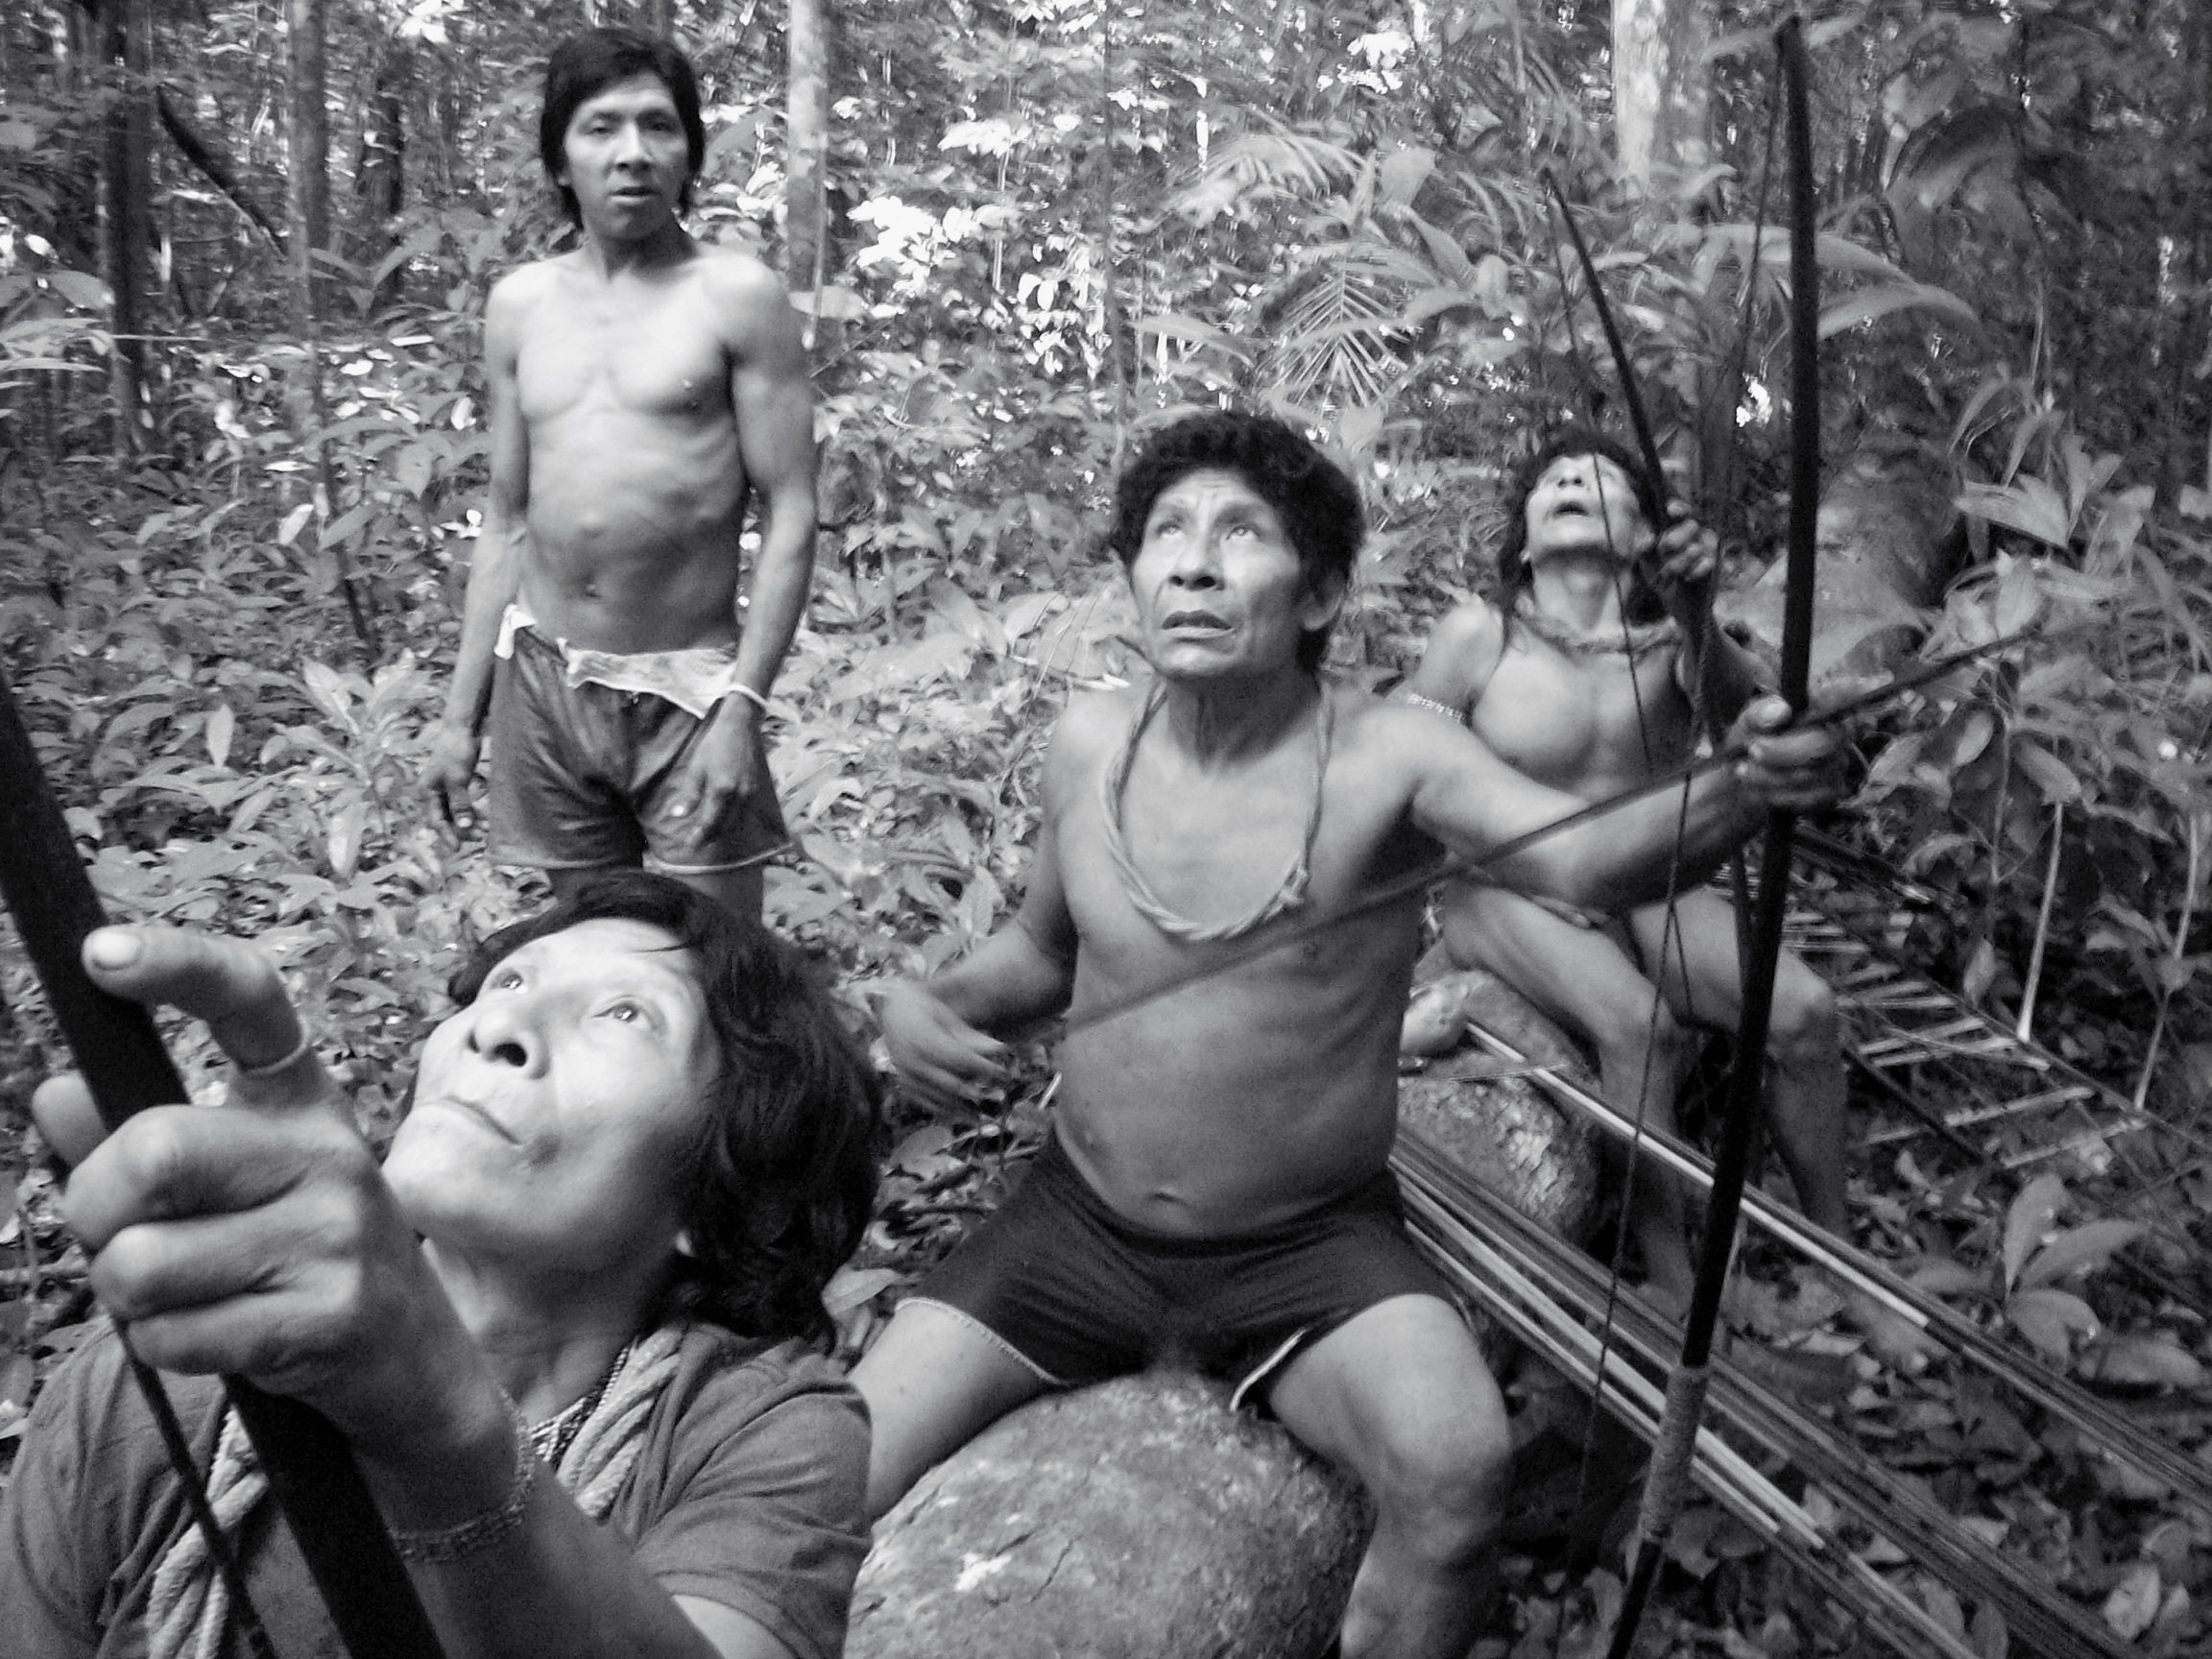
\includegraphics[width=\textwidth]{./imgs/100_5208}
\caption{Enquanto Uriximatỹa olha para a câmera, Kamará, Takya e Pirama’a observam a copa de uma árvore a procura de macacos (aldeia Juriti, 2007).}
\end{figure}

Na subida de uma árvore, é importante para quem for espantar os capelães
estar preparado para o inesperado, pois os animais podem correr antes
mesmo de o homem chegar; ou podem permanecer camuflados durante horas,
entre as folhas mais altas da copa, onde o caçador não conseguirá
alcançá"-lo, pois corre o risco mesmo de cair de uma altura de até 30
metros. Por meio do silêncio e da camuflagem, que lhes fornece alguma
segurança, os animais, muitas vezes, conseguem fazer com que os homens
duvidem de que estejam lá (como muitas vezes ocorreu). Nessas horas, os
capelães ficavam tão quietos que todos tinham dúvida se havia ou não
animais escondidos. O processo pode durar muitas horas, e os animais
podem (sim) vencer o caçador pelo cansaço. Nesse dia, especificamente,
Takya passou cerca de 20 minutos ``desafiando'' os animais, que em dado
momento se apavoraram com as palavras e fugiram. No momento imediato à
fuga, escutei muitos tiros, misturados a gritos, zunidos de flecha e
rugidos desafiadores. Após alguns segundos, os animais começaram a cair.
Alguns morrem quando são alvejados, outros morrem na queda, e há aqueles
que caem convulsionando, sangrando pela boca e emitindo sinistros
rugidos de desespero. A estes últimos são reservadas pauladas na cabeça
e no resto do corpo, dadas por crianças ou mulheres que cheguem ao
local. Um forte cheiro de urina empesteia o ar (como o cheiro de um
zoológico), pois, como tantos outros animais, os capelães também urinam
na hora da morte.

Neste bando havia sete capelães, sendo que cinco foram abatidos
(contando um filhote não muito pequeno e que, por isso, não ``prestaria''
para animal de criação). Enquanto Takya gritava com os animais no alto
da árvore, as mulheres em solo puxavam longos cipós que caíam até o
chão, para chacoalhar a folhagem da árvore onde estavam escondidos os
animais (muitas vezes, elas obtêm bons resultados com essa operação).
Mulheres mais velhas (como presenciei em uma caçada na aldeia Tiracambu)
podem, do solo, ``espantar os capelães'' proferindo as mesmas palavras que
os homens, e auxiliam quem estiver no alto (\emph{wate}), batendo palmas
e assobiando. Desconfio que o verbo \emph{papopo} tenha o nome \emph{po}
``mão'' incorporado, atestando esses bateres de palma. Depois da caçada,
todos se sentam para limpar suas espingardas, arcos e flechas; os mais
jovens verificam os cartuchos, enquanto os velhos reparam suas flechas
com a mesma preocupação que os jovens preparam novas cargas de munição.
Neste dia, especificamente, Muturuhũ matou dois capelães com suas
flechas; Wirahoa matou uma fêmea (e seu filhote) com sua espingarda; e o
(na época) jovem Kaawi'ia --- também com sua espingarda --- matou um macho.
Kamara se cortou bastante nos galhos, na descida de uma árvore. Ao
final, todos avaliaram seus ferimentos e esperaram o suor secar, com uma
conversa muito animada.

O \emph{wari} \emph{papopo} (``espantar o capelão'') é uma técnica
bastante eficiente e compõe o aparato de caça Guajá. Ainda assim, muitos
animais conseguem furar o cerco montado pelos humanos, seja porque o
caçador errou seu tiro (\emph{ajapi jawy}, lit ``errei o tiro''.), seja
porque o animal conseguiu fugir por um ponto cego, onde não havia
caçadores à espreita. Caso um capelão fure o meticuloso cerco de caça
(como ocorre com frequência), todos os que estão envolvidos na ação se
mobilizam ainda mais: as crianças correm, as mulheres gritam ``eles estão
aqui, não os deixem fugir''!, os cachorros latem e os homens, sempre
silenciosos e controlados, descem das árvores e correm em direção às
outras, para onde fugiram os sobreviventes. Mais um pouco, e podemos
ouvir tiros e mais barulhos secos de corpos caindo de alturas de 15 a 20
metros sobre o tapete de folhas que compõe a floresta.
\\

2.

Como estamos vendo, trata"-se de uma emboscada aérea. Os animais devem
ser surpreendidos para que não possam escapar. Em seguida, devem ser
espantados para que, ao fugir, literalmente se atirem contra os
caçadores. Por isso, tais emboscadas são bem"-sucedidas se realizadas nas
primeiras horas do dia, quando os capelães ainda estão dormindo. Nenhum
outro animal de caça (\emph{ma'amiara} --- caça, presa, bicho) tem essa
prerrogativa como necessária, a não ser os capelães. Se os homens os
rastreiam ainda pela manhã, a caçada se dá imediatamente. Porém, se
ocorre de encontrarem seus vestígios no final da tarde, sabem que se
instalarão em uma árvore para ``cantar'' e dormir, pois, diferentemente
dos macacos, os capelães não saem à noite para caçar (\emph{wata}) como
``doidos'' (\emph{waky}).

Ao identificar a árvore onde os bugios se instalaram, o homem que a
achou volta para a aldeia --- ou acampamento --- onde estão seus
companheiros e os chama para, no dia seguinte, os abater. Este indivíduo
quase sempre poderá receber uma grande parte do todo abatido, por ter
sido ele quem descobriu os animais. Ele é quem ``puxa'' (\emph{myty}) a
caçada, o \emph{tamỹ}, que toma a frente da empreitada e para quem,
muitas vezes, um homem (por algum tipo de serviço como um ``serviço da
noiva'') estará caçando. Muitas vezes, os homens --- aparentados
diretamente ou não --- podem ajudar um caçador que tenha encontrado um
grupo de capelães sem que recebam qualquer animal em troca. Esse
propositor da caça é o \emph{tamỹ}, tal como já vimos aqui.

O mais impressionante da caça aos capelães (e macacos em geral) é que
estes se locomovem pelas copas das árvores e, ainda assim, os humanos
conseguem cercá"-los e até persegui"-los pelo alto. Boa parte do sucesso
dessa caçada se deve às estratégias de emboscada aérea e ao domínio de
subir em árvores e cipós, independentemente do grau de dificuldade que
essas atividades impliquem. Os Guajá, por exemplo, nunca se conformariam
em deixar um primata enganchado entre os galhos após o abate, por mais
difícil que seja sua captura --- como na cena descrita por Descola em que
um Ashuar, conformado, deixa para trás um macaco"-barrigudo preso no alto
da árvore ``para os urubus'' (Descola, 2006, p. 155). Caso fiquem
enganchados entre os galhos com seus rabos e membros, como é comum, e se
a árvore for inacessível, sobem em outra próxima e tentam, pelas copas,
chegar até eles. Cortam varas com até cinco metros para alcançar o corpo
do animal enganchado (como se este desafiasse o caçador ainda depois de
morto). Pude presenciar algumas situações em que pensava ser impossível
que pudessem recuperar o cadáver resistente de um macaco ou capelão. E
lá estava o caçador, surpreendendo"-me, lançando galhos, subindo em
outras árvores, pendurando"-se em cipós. Tudo isso para que os primatas
fossem para o moquém e não virassem ``comida de urubus'' (\emph{uru}
\emph{nimi'ũa}).

Gosto de pensar que a caça em geral, e a caça de macacos em particular,
acaba por produzir uma crítica a noções caras a nós acerca de
\emph{animal} e \emph{espécie}. A caça conecta \emph{pessoas} e
\emph{animais} a partir de relações que ora passarão pela criação, ora
pelo abate, mas que nunca serão concomitantes, tal como ocorre conosco
em casos como a criação de bois e galinhas. Em outras palavras, tal como
sabemos, o que se cria não se mata, o que se mata não foi criado, e isso
pode não ser trivial. Certa feita, um amigo abatera um macaco"-prego com
um tiro na parte traseira do crânio. O cérebro do animal ficara exposto,
e mesmo depois de horas após a caçada podíamos ouvir no pátio de nosso
acampamento o bicho moribundo lutando para não morrer. Lembro que aquela
cena me atormentou, acabei pedindo para que alguém terminasse de vez com
o animal para aliviá"-lo (ou me aliviar) de tanto sofrimento. Foi quando
todos que me ouviram desataram a rir, não sem acatar os meus apelos.
Sobre o animal, além de me mencionarem uma ideia que alguns guajá
defendem e que nunca entendi direito, a de que ``bicho não sente dor''
(\emph{nikaj hahyha}, ``não sente dor''), o outro comentário que me
fizeram, entre muitas risadas, era o fato de aquele macaco resistente
ser parecido com os ``brancos'' e ser difícil de matar (``de morrer'',
para ser mais preciso). Tal maneira de pensar macacos como animais de
caça é estranha a mim, pois somos informados pela nossa primatologia,
pelo nosso etno"-conhecimento, de uma continuidade lógica e inseparável
entre nós e os primatas, algo que os Guajá não compartilham. Meus amigos
neutralizam isso muito facilmente retirando não só os macacos, mas todos
os animais caçáveis dessa linha de continuidade interespecífica --- do
tipo ocidental ``somos todos animais'' ---, o que faz tudo mudar. É como
se, para os Guajá, a \emph{caça}, como um modo de interação, em nada
tivesse a ver com a \emph{domesticação} de animais, como outro modo.

A tônica, portanto, não recairá na \emph{espécie} (tal como nós
concebemos cachorros como um tipo de animal e jaguatiricas como outro),
mas em distintas formas de relação; ou, podemos pensar, diferentes
afecções. Como se os animais de um tipo (caçados) tivessem pouca relação
com animais do outro tipo (criados), mesmo sendo um da mesma
\emph{espécie} que o outro. A natureza das interações entre humanos e
animais, na caça e na domesticação, são não apenas de universos
diferentes, mas a própria ideia de \emph{animal} pode não ser informada
pela ``animalidade'' de certas espécies em oposição a ``domesticidade''
de outras, mas pela forma com que os Guajá se relacionam com esses
bichos. Por exemplo, tal como outros povos amazônicos, os Guajá não têm
uma palavra para \emph{animal} \emph{genérico} (ver p. ex. Vander Velden,
2012, p. 238), mas guardam uma para animal `\emph{caçável'}
(\emph{ma'amiara}) e outra para animal `\emph{criável'} (\emph{hajma}).
Por esta lógica, um macaco"-prego na floresta pode vir a ser mais
perigoso do que uma onça doméstica (e as pessoas lembram todo o tempo o
quanto os macacos"-pregos são agressivos e ``doidos''), não havendo um
\emph{a priori} de agressividade da espécie, embora os Guajá defendam
que, no mato, uma onça (quase) sempre será mais perigosa que um macaco.

Se essas duas características são indissociáveis, como sabemos da caça
amazônica, no caso Guajá uma se vincula diretamente à outra, em que a
comida e a criação são condicionantes entre si, operando algo como um
\emph{duplo vínculo}, tal a célebre formulação de Gregory Bateson, pela
qual, o que quer que se faça para se desvencilhar, não há como vencer
(1956 {[}2000{]}): para os Guajá criarem precisam matar, para caçarem
precisam cuidar. É comum ver homens que saem para o mato para caçar
dizerem a suas filhas que trarão como regalo um filhote de macaco ou de
cotia, produtos da caçada que farão. Também vemos meninas que desatam a
chorar por não terem um animalzinho de criação serem consoladas por seus
pais e mães que prometem lhe trazer um quando houver uma nova caçada. Os
homens Guajá reclamam que suas crianças choram querendo filhotes de
macaco e cotia para criar. Sendo assim, e como sabemos de tantos povos
amazônicos, na mesma jornada que se produz comida na forma de caça são
capturados os animaizinhos de estimação. Porém, diferentemente de
concluir que a criação desses seres funcionaria como uma compensação
pela morte de seus semelhantes caçados, como outros autores o fizeram,
no que concerne a diferentes animais --- comidos e criados --- esse fenômeno
parece recolocar a própria ideia de \emph{espécie} como algo dado. Ao
menos sob a perspectiva humana, parece que estamos diante de diferentes
\emph{tipos de animais}, por assim dizer, que aparecem como efeito de
relações (repito, ao menos para os humanos). Não apenas o próprio bicho,
mas o tipo de relação importaria tanto quanto a espécie do animal. É a
\emph{relação}, se assim posso colocar, que parece primária aqui, seja
no tratamento cuidadoso dos animais criados, seja na forma ``impiedosa''
que reservam aos animais caçados. Neste caso, a própria noção de
\emph{espécie} (que, como sabemos, está em debate há pelo menos 150 anos
na biologia --- Haraway, 2003, p. 15) seria subordinada a esse \emph{duplo
vínculo}, não havendo a \emph{espécie} em si, mas ``agenciamentos'' de
caça e outros de criação. Para esta etnografia, são esses diferentes
modos de relação que interessam, e não os bichos, espécies, gêneros,
ordens ou classes em si.

\section{Entre o rastro e o som: a poética da predação}

Os Guajá dificilmente caçam os capelães no final da tarde, hora em que
os animais estão ``cantando''. Ao contrário, ao perceber os capelães
cantando, param para ouvi"-los, e, pelas vozes, conseguem distinguir
quantos são fêmeas ou machos; adultos ou filhotes. E então traçam planos
para o dia seguinte, quando os perseguirão. Certa tarde, eu andava com
Pira'ima'ã na floresta quando ouvimos um grupo de capelães entoando seu
som característico. Com o que ouviu, ele conseguiu todas as informações
de que necessitava para o dia seguinte: tratava"-se de uma fêmea
solitária com dois filhotes em uma copa, enquanto o resto do grupo
estava um pouco mais distante. Ele me explicou que o som emitido pelas
fêmeas é mais delicado do que o do macho, que tem um ``canto'' grosso. Em
outra situação, ao ouvir sons de capelães comentei com Ajruhua sobre o
canto. Ela me respondeu que eram filhotes e que não estavam cantando
(\emph{jã}), mas sim, chorando (\emph{ja'o}), pois quem cantava eram
apenas os adultos da espécie. Escutar (\emph{nũ}) o som"-canto
(\emph{jã}) dos animais é fundamental para as caçadas, sobretudo de
capelães. Sentenças como ``vamos caçar capelães amanhã, pois alguém os
ouviu cantar naquela direção!'' ou ``vamos sair para escutar os
capelães!'', dentre tantas outras formas, associam o som"-canto do capelão
com a busca pelo animal. Em outras palavras: \emph{é preciso saber
escutar os capelães para poder caçá"-los} (além de outras presas). Pelo
canto dos capelães, sabe"-se a quantidade e a diversidade do bando, tal
como a pegada de um animal terrestre revelará seu peso, idade, sexo e
outras informações relevantes.

Ouvir os capelães pode ser encarado como uma ``estratégia de caça'', mas
sabemos há algum tempo que as ``estratégias'' de povos como os Guajá
(caçadores, por excelência) não se resumem a um jogo de sobrevivência e
forrageio. Suas práticas de produção da vida estão longe de um aspecto
comportamental ilógico, pois não podemos reduzir as atitudes dessas
pessoas a um economicismo que tende a naturalizar (no sentido de colocar
no plano da Natureza) as atividades de caça, coleta, dentre outras
(Ingold, 2000, p. 58). Os Guajá, por exemplo, param para escutar os
capelães independentemente de caçá"-los ou não, pois (como sempre
afirmam) ``gostam'' (\emph{maparahy}) do canto deles e sempre que podem
elogiam a capacidade que tais animais detêm de ``cantar bonito''
(\emph{jã} \emph{paryhỹ}). Para as pessoas da aldeia Juriti, eu sempre
deveria gravar o canto dos capelães com a mesma assiduidade com que
gravava o canto humano e com o mesmo objetivo: levar para São Paulo e
mostrar aos outros brancos como os \emph{awatea} (as pessoas), mas
também os capelães, ``sabem cantar'' (\emph{kwa} \emph{janaha}). É claro
que muitos animais conseguem cantar (os pássaros são o maior exemplo
disso), mas os capelães eram os únicos que lhes interessavam gravar.
Foram muitas as vezes em que pudemos ouvir, de muito longe, no final da
tarde, capelães produzindo seus sons característicos. E sempre havia
alguém pedindo para que eu gravasse seus rugidos. Eu, gentilmente,
atendia ao pedido, mas apenas para mostrar que o sons da aldeia
(crianças, galinhas, cachorros) e os sons da floresta (vento nos galhos,
assobios de pássaros e outros animais) se interpunham entre o gravador e
o canto dos capelães, o que não permitia que o canto, que estava longe,
fosse bem registrado.

Sem dúvida, ``ouvir'' pode ser uma das melhores formas de conhecimento
quando as pessoas vivem na floresta, como é o caso de diversos grupos
amazônicos. Com o campo de visão limitado e a necessidade de não serem
vistos, a espreita e a escuta são formas extremamente adequadas a essa
realidade\footnote{Como escreve Cabral de Oliveira para os Wajãpi, ``O
  ouvido atento é marca de um bom caçador'' (2012, p. 97).}.

Porém, os Guajá sugerem que a caça em si (como continuaremos vendo)
oferece outras sensações aos humanos. E, por mais contraditório que isso
possa parecer para a nossa tradição de pensamento (que tende a separar
algumas espécies animais para se afeiçoar, enquanto outras são para
consumir)\footnote{Ou, como observa Erikson: ``\emph{nous nous efforçons
  de séparer radicalement le familier et le comestible, alors que les
  Amazoniens sont pour leur part soucieux d'un juste équilibre entre les
  deux}'' (Erikson, 1997, p. 03).}, o fato de as pessoas gostarem da música
dos capelães é o mesmo que os faz gostar de os matar. Criá"-los e
caçá"-los não são aqui duas formas de relação tão diferentes entre si.
Vejamos melhor esta suposição.

Talvez tenha sido Ingold quem melhor observou que, entre muitos povos
não ocidentais, e em particular os chamados caçadores"-coletores, ``a
diferença entre as atividades de caça e coleta, de um lado, e cantar,
narrar estórias e mitos, de outro, não podem ser postas em termos de uma
dicotomia entre material e mental, entre interações ecológicas \emph{na}
natureza e construções culturais \emph{da} natureza'' (Ingold, 2000, p.
57). Para o autor, ``ao contrário, ambos os conjuntos de atividades são,
antes de tudo, maneiras de habitar {[}no mundo{]}
(\emph{dwelling})''\footnote{Para o sentido exato da ideia de
  \emph{dwelling} \emph{perspective} --- um conceito central nas análises
  de Ingold ---, ver Ingold, 2000, pp. 153--156.}. Trata"-se de um
``envolvimento poético'' (nas palavras desse autor) que, no caso Guajá,
sugere que caçar não é apenas conhecer (espécies e hábitos animais), mas
se engajar com tais espécies, habitando um mundo em que a caça ganha
elementos da ``guerra'' e os animais não são coisas destituídas de
``alma'' ou personalidade. Hugh"-Jones observa que o idioma da guerra é
utilizado por grupos do noroeste amazônico, sobretudo quando se referem
a caçadas coletivas. De acordo com o autor, os queixadas naquela região
encarnam a imagem do inimigo selvagem em ataque. E, ``embora toda caça
coletiva conote de uma maneira ou de outra a guerra, esse efeito é
ampliado de acordo com o número de queixadas'' (1996, p. 14). No caso
Guajá, encontramos também paralelos com essa ideia.

Os Guajá defendem que, ao emboscarem os capelães, os animais
\emph{falam} entre si: ``vamos embora, pois estamos cercados por
inimigos'' (\emph{mihua}), e \emph{inimigos}, nesse caso, deve ser
entendido como uma \emph{posição} ocupada pelos humanos, a partir do
ponto de vista dos capelães, para evocar aqui a noção de \emph{ponto de
vista} discutida na etnografia Yudjá (Lima, 1995, 1996, 2005). O tipo de
inimigo (\emph{mihua}) variará conforme o narrador da caçada e da
situação. O importante nessa ideia é que os animais apreendem os humanos
enquanto \emph{inimigos}, podendo ser \emph{madeireiros mihua}
(madeireiros"-brabos), \emph{karai} \emph{mihua} (brancos"-brabos) ou
\emph{awa} \emph{mihua} (gente"-braba). Isto é indiferente, pois o efeito
produzido na \emph{mente}\footnote{Refiro"-me à ``mente'' a fim de
  explicitar que os guaribas ``pensam'' (\emph{imarakwa} --
  pensar/imaginar) se tratar realmente de inimigos --- tal como os Guajá
  definem.} dos animais é o mesmo. A ideia"-imagem de \emph{karaia}
(brancos) como sinônimo de inimigo, por exemplo, é recorrente quando
comentam a relação entre a caça (\emph{ma'a}, ``presa'') e caçador
(\emph{watama'a} --- literalmente ``caminhador''). Quando relatam que certo
animal fugiu podem, em tom jocoso, dizer, modificando a voz, ``corram,
corram, os \emph{karaia} estão doidos e estão vindo nos matar, corram'',
e todos caem na gargalhada.

Um termo que entrou definitivamente para o léxico da língua Guajá é
\emph{índio}, que pode ser utilizado de diferentes maneiras. Na forma
``positiva'' o utilizam quando se referem à terra indígena: ``essa terra é
nossa, é terra de índio'' --- nesse caso, sinônimo de \emph{awatea}
(humanos). Ou quando queriam que eu entendesse a quantidade de pessoas
que habitavam o céu (\emph{iwa}) também diziam ter ``muitos índios''
(humanos). Porém, por ser uma ideia ``importada'' e bem maleável, também
pode aparecer como sinônimo de \emph{mihua} (inimigo) e vir ou não
acompanhada do adjetivo \emph{brabo} (``\emph{índio} \emph{brabo}''). Por
isso, durante as caçadas os capelães podem ser ditos \emph{índios};
nesse caso, um sinônimo para ``inimigo'' e/ou ``não"-semelhante''. Uma das
primeiras vezes em que ouvi se referirem desta forma foi durante uma
caçada de capelães (que acompanhei), quando os animais se anteciparam
aos caçadores e conseguiram escapar, deixando todos muito tristes. Em
seguida um homem veio falar comigo, ``\emph{índio} \emph{wyhy}'' (``índio
correu''), e os \emph{índios} em questão eram os capelães. Assim, para os
capelães os Guajá são \emph{madeireiros}, \emph{brancos}, \emph{índios}
(ou qualquer outro termo que ocupe a posição de inimigos) que irão
matá"-los, por isso fogem com seus filhotes.

Da perspectiva do animal predado, portanto, a caça é uma guerra em quem
os humanos (\emph{awa}) podem matar os animais (\emph{ma'amiara},
``presa''), e por isso eles enxergam os humanos como inimigos
(\emph{mihua}). O mesmo encontramos em exemplos paradigmáticos como na
etnografia Araweté na qual ``para os animais, os Araweté são \emph{awĩ},
inimigos --- exceto para a onça, que, ela é que é \emph{awĩ}, e nós seus
\emph{hẽmĩnã} (`presa'). É por isso que se dança sobre a morte de uma
onça como sobre a de um inimigo'' (Viveiros de Castro, 1986, p. 350).
Entre os Araweté pode ser encontrado algo próximo --- em conteúdo e forma
--- ao caso Guajá da caça aos capelães como uma caça extremamente
sociável. Viveiros de Castro observa:

\begin{quote}
\emph{Os queixadas e guaribas, certamente devido a seu costume de viverem em
bandos, são uma fonte rica de metáforas da sociedade para os Araweté, e
sobretudo da relação de guerra entre sociedades. Assim, eles sempre
comparavam a técnica de cerco kayapó com a que eles utilizavam contra as
varas de porcos; e gostavam de arremedar o pânico dos guaribas e porcos
quando atacados pelos caçadores; os bichos gritariam: `\emph{awĩ},
\emph{awĩ}!'. Os jabotis, por sua vez, são comparados a cativos de
guerra, por ficarem presos nas casas até serem mortos e comidos. A
associação entre caça e guerra é clara para os Araweté (como para os
Wayãpi --- \emph{cf}. P. Grenand, 1982, p. 208; 1980, p. 42) (Viveiros de Castro,
1986, p. 209)}
\end{quote}

É importante observar que a caça Guajá está baseada na ideia de que boa
parte dos animais enxergam os humanos como inimigos (\emph{mihua}). É
isso que orientará as técnicas de caça, pois os humanos caçam seres que
(sabem) os percebem como inimigos. Mais do que isso, pois, se em linhas
gerais podemos afirmar --- parafraseando Lima --- que ``aquilo que os humanos
apreendem como caça, os capelães\footnote{A autora se refere a
  \emph{porcos}, e não a capelães.} apreendem como guerra'' (1996, p.
34); a perspectiva da guerra não pode ser relegada ao mundo animal,
quando os humanos apenas ``caçam'' e os animais ``combatem''. Os humanos
precisam utilizar um arsenal simbólico"-guerreiro para fins
ecológicos"-alimentares. ``Caçar capelães'', portanto, além de se basear no
ato de ``espantar o capelão'' (\emph{wari} \emph{papopo}), é
potencialmente uma atividade de \emph{ha'a waria}, ``enganar o capelão'',
e isso é feito de forma muito consciente, em que os humanos aproveitam o
fato de serem vistos pelos animais como \emph{inimigos}. Podemos pensar
que, se durante uma caçada os humanos são vistos como inimigos
(\emph{mihua}) aos olhos dos animais, é porque também eles \emph{se
tornam capelães para caçar} e guerrear com outros --- agora --- parcialmente
``iguais'' (ao menos para esse fim estratégico). Muitas das caçadas
guajá estão baseadas na imitação (gerada por um profundo conhecimento
dos hábitos animais); os homens precisam falar a língua dos capelães
para que eles pensem que se trata de algum tipo de ser próximo (seja um
parente distante, \emph{harapihianã}, ou um inimigo, \emph{mihua}, isso
não importa muito).

Parte da habilidade do caçador é apoiada nessa capacidade de
``mimetismo'', tal o sentido que Willerslev (2007) empresta ao termo. Em
sua etnografia sobre os Yukaghirs, um povo da Sibéria Oriental
(caçadores de alces e renas; produtores de pele; e detentores de uma
técnica apurada para a caça desses animais, que --- pelo uso de peles,
gemidos e movimentos --- se ``transformam'' em alce a fim de os caçar),
Willerslev introduz um problema análogo ao que encontro aqui, porém em
uma paisagem etnográfica muito distante. De acordo com o autor, a caça
de alces Yukaghirs propõe uma equação de difícil resolução, uma vez que,
ao se passar por alces, os homens experimentam uma situação liminar,
pois, se um caçador não é propriamente um alce, ele também ``\emph{não} é
um alce'', ocupando ``um estranho lugar entre as identidades humanas e
não"-humanas'' (Willerslev, 2007, p. 1). Pensando a partir dessa ideia, a
imitação envolvida na cinegética Guajá funciona não como uma forma de
representação que os caçadores descobriram apenas para assustar os
capelães, mas sim como uma forma de relação assimétrica cujo polo é
marcado por um exercício de poder guerreiro, de caçadores sobre essa
espécie, cujo objetivo final é a predação (ver Willerslev, 2007, p. 11).
A fala do capelão é vista na boca humana, e se não acontece uma
metamorfose de um no outro, humanos tentam transformar um tipo de
perspectiva que os outros (os capelães) têm sobre eles (os humanos). A
questão, tal como discutido por Willerslev, é que os ``caçadores irão
experienciar os animais como pessoas a partir de um ponto de vista
similar, mas não idêntico ao deles (dos animais) (2007, pp. 98--99).

O autor não deixa de mencionar que o fato de um caçador ser como a presa
faz dele, sem dúvida, uma estranha presa, pois --- por mais semelhança que
ele tente estabelecer com o animal a ser caçado (um registro sonoro, no
caso Guajá; ou visual como no caso Yukaghir) --- as diferenças reais entre
caçador e presa continuam sendo incomensuráveis. Por mais que um caçador
guajá queira (embora eles não queiram), nunca se parecerá inteiramente
com um capelão, pois a identificação mimética entre um caçador e sua
presa não é mesmo para ser \emph{total}, porém \emph{parcial}, e é
justamente essa pequena diferença sobre o mundo representado que faz com
que o caçador exerça poder sobre essa presa, pois, ``sem diferença,
imitador e imitado entrariam em colapso, um se tornaria o outro,
tornando qualquer exercício de poder algo impossível'' (Willerslev, 2007,
p. 11)\footnote{Essa também será a definição de Pendersen para
  \emph{animismo}, formado por identificações análogas, ou parciais, e
  não totais (Pendersen, 2001 \emph{apud} Willerslev, \emph{op. cit}., p. 24)}.
Citando"-se novamente o etnógrafo siberianista: ``O caçador sabe, ou ao
menos deveria saber, que o alce e ele não são exatamente os mesmos''
(2007, p. 99). Além disso, tornar"-se um outro animal é, como sabemos há
algum tempo, uma das piores catástrofes que se podem abater sobre a
pessoa, tanto ameríndia (Seeger \emph{et al.}, 1979; ver também Viveiros
de Castro, 2002, pp. 390--391) quanto na Sibéria (Willerslev, 2007,
pp. 99--100). Trata"-se, para a caça de capelães, de uma metamorfose
corporal, porém de risco calculado, pois fica óbvio que os Guajá não
colocam sua relação com os capelães em níveis simétricos. Ora os
capelães são animais de criação (\emph{nima}), ora são comida
(\emph{hami'ũa}). Antes de comida, caça (\emph{ma'a}). E para que sejam
caçados se tornam inimigos (\emph{mihua}). Serão sempre relações que
envolvem assimetria --- termo mais adequado à paisagem amazônica do que
``poder'', como proposto por Willerslev para a Sibéria. Assim, fazer com
que os capelães pensem ser o caçador um igual, ainda que inimigo
(\emph{like"-me"-but"-not"-me}, Willerslev, 2007, pp. 98--99), é um ponto de
destreza ao mesmo tempo que uma condição da atividade de caça.

Ingold se reporta a uma ``economia cósmica de compartilhamento''
(\emph{cosmic} \emph{economy} \emph{of} \emph{sharing}), em que animais
e plantas mantêm com os humanos uma relação de ``parceria'' --- embora entre
os Guajá estejam ausentes características de ``devoção'' à ``mãe da caça''
ou ao ``espírito do vento'' que propiciam uma boa caçada, como vemos em
caso de caçadores do ártico e subártico, além de em outros casos
amazônicos (ver Ingold, 2000, p. 48 e Descola, 2005, pp. 459--496 para
exemplos diversos; e Descola, 2006, p. 172, pra um caso amazônico). Para
diversos grupos, observa Ingold, a caça deve ser ``encarada não como uma
manipulação técnica do mundo natural, mas como uma espécie de diálogo
interpessoal, parte integrante de todo o processo da vida social em que
pessoas humanas e animais são constituídos com suas identidades e
propósitos'' (Ingold, 2000, p. 49). O que encontramos aqui entre os Guajá
é um certo ``padrão amazônico'' para caça, em que elementos de guerra são
reais também para a atividade caçadora --- no sentido de uma ``confrontação
coletiva'', tal como prescreve Descola para os conflitos, sejam de caça
ou de guerra, na Amazônia (1993, p. 171; 2005, p. 461), e que no caso
Guajá envolve vingança, resguardo, dentre outros elementos que veremos
aqui.

Além das habilidades e equipamentos necessários, conforme já demonstrado
aqui, toda a caça de capelães e boa parte da lógica da predação animal
Guajá está baseada em induzir a caça ao erro, ``enganar a caça''
(\emph{ma'amiara} \emph{ha'a}) como afirmam os caçadores. Um bom caçador
é aquele que, a partir das técnicas certas (silêncio, imitação,
rastreamento), faz com que o animal caçado se confunda e cometa erros
que não cometeria em uma situação de ``equilíbrio'' (como na ausência do
caçador, por exemplo). Os Guajá imitam com perfeição grunhidos e
assobios de diversos animais --- muitos dos quais não são caçados ---, e
essas imitações aparecem para ilustrar de forma magnífica as narrativas
noturnas sobre as caçadas (chamadas \emph{mumu'ũha ``narração''}). Tais
imitações, porém, extrapolariam a barreira estética (apesar de seu
realismo e beleza) e são também uma forma de conexão com a presa,
formando algo como uma \emph{poética da predação}. O caçador Guajá é,
nesse caso, uma espécie de influenciador que se disfarça entre as
folhagens e, com assobios e gemidos característicos de cada animal,
consegue confundir a presa, atraindo"-a para a morte, quando a faz pensar
tratar"-se de um semelhante. Para caçar é necessário que se comuniquem
(\emph{ma'i} ``falar''; ou \emph{hamakaj} ``chamar'') com os animais por
meio desses chamados específicos. Tal comunicação é chamada \emph{ha'ỹ
hanima}, ``chamar o meu animal de criação'', o que acena para uma relação,
ao menos liminar, entre ``animais de caça'' e ``animais de
criação''\footnote{Ha'ỹ é mais do que ``chamar''. Além de ``imitar'', o
  mesmo verbo é utilizado também com o sentido de
  ``experimentar/tentar'' para quando querem comer uma comida nova ou
  tentar fazer algo que nunca fizeram. Um sentido mais geral para esse
  verbo, que englobe essas noções, pode ser algo do tipo ``fazer
  igual''.}. Neste caso, caçadores utilizam recursos miméticos para
ludibriar suas presas, fazendo"-as acreditar que, em vez de matadores, os
sons são provenientes de seres de seu universo ``familiar'' (os
\emph{hapihiara}, ``parentes próximos'', diriam os Guajá; ou mesmo os
\emph{jara}, donos de animais de criação). Nesses momentos, as
diferenças entre animais de criação (\emph{hanima} --- ``meu animal de
criação'') e de predação (\emph{hama'a} --- ``minha caça'') estão suspensas,
visando a melhor estratégia (guerreira) de caça. Uma presa
(\emph{ma'amiara}), portanto, pode ser tratada, mesmo que por um
momento, como um animal de criação, em um chamamento suave, um som
confiável, feito para enganá"-la. Aquilo que aos ouvidos dos animais é
fala ou canto (\emph{poética}) é, por uma inexorável verdade, o
prenúncio da morte (\emph{predação}).

Para o veado (\emph{arapaha}), emulam um gemido anasalado,
``\emph{mẽẽẽ}'', idêntico ao que é produzido por este cervídeo. Assim, o
animal pensa (\emph{imarakwa}, ``pensar"-imaginar'') tratar"-se de um
outro de sua espécie. Para a cotia (\emph{akwixia}), produzem um som
aspirado, principalmente quando não a encontram ou quando o animal está
em fuga. Ainda conseguem imitar o som de filhotes de cotia, para
ludibriar adultos da espécie e os atrair. Quanto a esta última
possibilidade, reescrevo um depoimento de Wirahoa que me foi concedido
em 2008:

\begin{quote}
\emph{Ao encontrar uma cotia prestes a fugir, se a chamo, imitando o som de
um filhote, ela pensará que os ``brancos'' (\emph{karaia}, nesse caso
sinônimo de ``inimigos'') aprisionaram seu filhote. Ao ouvir o meu
chamamento, a cotia bate suas patas no chão em desafio, como se
pensasse, ``o que esses \emph{karaia} estão querendo ao aprisionar o meu
filhote?''. Com isso consigo deixá"-la com dúvida, se questionando sobre a
veracidade dos choros que está ouvindo. Enquanto ela está parada,
``pensando'', eu atiro e a mato. Então, ao morrer ela pensa, ``não havia
nenhum filhote aprisionado; foram os \emph{karaia} que me enganaram, só
para comerem minha carne''}.
\end{quote}

Este exemplo é interessante também para notarmos que, de acordo com essa
teoria guajá --- que é, de muitas maneiras, perspectivista ---, os caçadores
nunca serão \emph{awatea} (gente) para os animais caçados. Se as presas
pensam, e caso tomem os caçadores por algum tipo de humano, estes
últimos encarnarão justamente os \emph{karaia} (não indígenas),
justamente o tipo de gente que os Guajá, apesar de viverem próximos hoje
em dia, tendem a evitar.

Antes de seguirmos para outro exemplo, lembro que, diferentemente dos
capelães, que roncam, os outros \emph{macacos} (macaco"-cairara, cuxiú e
macaco"-prego, ou \emph{ka'ihua}, \emph{kwixua} e \emph{ka'ia}
respectivamente) contam não só com gritos estridentes que lhes servem de
proteção, mas também com assobios, com os quais os indivíduos de um
bando se comunicam. Embora a técnica de ``espantar o capelão'' possa ser
utilizada para a caça de macacos em geral --- como presenciei por diversas
vezes, quando os bandos de macacos se escondiam na copa de uma árvore e
os caçadores alcançavam o mesmo sucesso que obtêm com os capelães ---, os
assobios dos outros \emph{macacos} também podem ser imitados pelos
humanos. Enquanto com os capelães a técnica específica é o \emph{papopo}
(espreita e espanto), quando se trata de macacos os caçadores podem
mimetizá"-los de outras formas, sobretudo por meio dos ``diálogos''
assobiados que os diversos primatas, como os macacos"-pregos, travam.

Na caça aos diversos tipos de macacos, os assobios característicos
emitidos pelos primatas em sua comunicação são reproduzidos por um
caçador a fim de os ludibriar e (\emph{ha'a}) e matar (\emph{ika}), como
ocorre com outras presas. Um dos momentos em que isso apareceu de
maneira vívida foi durante uma caçada com Wirahoa. Nesse dia, ele me
propôs: ``vamos caçar!'' ( \emph{are xiwata pyry!} --- ``vamos andar
junto!''). Saímos sem cachorro ou qualquer outra companhia. Somente nós
dois, com um pouco de comida (algumas bolachas e um naco de fígado de
jaboti assado) e a promessa de matarmos alguns macacos"-pregos que seu
irmão havia rastreado no dia anterior. A certa altura da caminhada,
ouvimos um bando deles se comunicando. Nessa hora, Wirahoa pediu"-me que
ficássemos parados onde estávamos e começou a assobiar (\emph{opia}) um
silvo característico, a fim de chamar os animais. Enquanto assobiava, os
macacos respondiam. Era verão, e Wirahoa me pediu para andar de forma
leve, para que o barulho das folhas secas remexidas não espantasse os
animais. Foi nessa hora que ele reforçou ser por isso que os Guajá
caminham descalços na floresta: para andar em silêncio (ao invés de
descalço, eu calçava uma desajeitada botina que protegia meu ``pé mole'',
\emph{ipya} \emph{memeka}, como me falavam os Guajá). Wirahoa me
explicou que aqueles assobios fariam com que os macacos"-pregos
(\emph{ka'ia}) pensassem se tratar de \emph{harapianã} (``cunhados''),
parentes distantes que vieram encontrá"-los e que, por isso, parariam
para ouvir e até mesmo poderiam vir em nossa direção. Não foi sem
surpresa quando chegou a meus ouvidos o som de folhas se remexendo na
copa de uma árvore a alguns metros de distância de nós. E lá estavam os
macacos, que continuavam ``dialogando'' com Wirahoa --- agora um (\emph{awa}
que se comunicava com a voz de um) macaco"-prego. Eles ali permaneciam,
nos galhos, à vontade, como se a morte não fosse iminente. Por isso
Wirahoa conseguiria matar confortavelmente um ou dois macacos, sem
sequer ``trepar no pau'' (\emph{irá} \emph{ipi} --- ``subir na árvore'').
Quando os animais pressentiram que estavam sendo enganados,
amedrontaram"-se e fugiram pulando de galho em galho. Ainda os seguimos
por um longo trecho, mas eles conseguiram sumir no meio da mata.

Além dos assobios, gemidos e ruídos, as pessoas confeccionam alguns
apitos, com taquaras e outras plantas com formato tubular, para atrair
caças. Esses objetos, chamados \emph{hamakajha} (``instrumento de
gritar''), podem reproduzir, por exemplo, o som de uma anta (um silvo) ou
de galináceos. No caso da anta, sabemos que os machos assobiam para
atrair as fêmeas da espécie. Segundo os Guajá, ao utilizarem o
\emph{hamakaj} o animal pensa tratar"-se de um parceiro/parceira à
procura da cópula (\emph{iminũ} --- ``fazer sexo''). Se a anta se dispersa,
o caçador apita de forma encadeada, o que a faz parar, ``pensando'' se
tratar de um parceiro. Pude presenciar tal situação ao lado de
Juriximatỹa, um caçador que passou boa parte de nossa caminhada apitando
seu \emph{hamakaj}, pois seguia o rastro de uma anta. Ficamos muito
próximos do animal, que não percebeu que o apito era assoprado por um
humano, porém ela conseguiu escapar quando muitos homens se aproximaram.
Em outra ocasião, voltando à noite de uma caçada com Pira'ima'ã,
andávamos por uma trilha quando ouvimos um silvo de anta. Ele comentou:
``Está ouvindo? É uma anta procurando fêmea para copular. Ela está vindo
 em nossa direção. Vamos esperar aqui para ver o que acontece!'' Eu
perguntei se era mesmo uma anta, já que estávamos em um \emph{awa}
\emph{pea}, uma ``trilha'' aberta por humanos e evitadas pelos animais de
caça. Então me respondeu em português: ``parece que é!''\footnote{Como já
  escrevi anteriormente, essa é uma expressão muito utilizada em
  português, ``parece que é'', e os Guajá raramente respondem uma pergunta
  com ``sim'' ou ``não'', mas com ``parece ser''. Na língua Guajá, a
  partícula epistêmica similativa \emph{rawỹ}/\emph{nawỹ} é muito
  utilizada. Indica algo que se supõe verossímil e pode ser traduzida
  como ``aparentemente''. O melhor exemplo está na pergunta ``\emph{o que
  é?}'', que na língua Guajá aparece como \emph{ma'a nawỹ} e deve ser
  traduzido literalmente por ``\emph{o que parece ser?}'' (para observar o
  funcionamento desta partícula na língua Guajá, ver Magalhães \emph{op. cit}., p. 116).}. Instamos por algum tempo e, de longe, avistamos uma lanterna.
O silvo se tornava ainda mais forte e percebemos se tratar do grupo de
Hajmakoma'ã que --- também voltando de uma caçada --- ainda apitava, com a
esperança de encontrar uma anta cujo rastro haviam encontrado na mata.

Logo na minha primeira ida a campo, comprei um violão em São Luís para
que me acompanhasse na viagem. Junto com o violão comprei um diapasão de
sopro que reproduz o som das seis cordas do instrumento. Ao conhecerem o
afinador, alguns homens se mostraram muito interessados, principalmente
pelas três notas mais agudas (Sol, Si e Mi) que, segundo alguns me
explicaram, era um bom instrumento para atrair aves como o jacu
(\emph{jakua}) e o inhambu"-galinha (\emph{iramua}), devido à variação
dos sons. Após alguns dias, Pira'ima'ã pediu"-me para dar"-lhe aquele
\emph{hamakaj} (``apito"-chamador'') que reproduzia muitos sons. Caso eu
necessitasse afinar o violão era só lhe pedir ``emprestado''. E assim
fizemos, com a condição de que ele me chamasse para suas caçadas quando
fosse utilizá"-lo. Devido a essa troca, pude vê"-lo utilizar o apito
muitas vezes em caçadas, porém sempre sem sucesso. Quanto ao
mutum"-cavalo (\emph{mitũa}), que produz um som grave"-anasalado, imitavam
muito bem com a boca, enquanto para as pacas --- um animal muito caçado ---
não existe som característico que possam imitar, já que ela só emite o
bater de dentes nas coisas e outros grunhidos irreprodutíveis.

\section{\emph{O pensar} e a caça}

1.

Para compreendermos os processos de caça Guajá temos que entender que,
segundo a teoria Guajá e de acordo com um modelo ameríndio mais geral
(Viveiros de Castro, 2002; Descola, 2005), vários animais contam com
capacidade de raciocínio, tal como os humanos. Vale lembrar que
\emph{imarakwa} (termo já discutido anteriormente) é o verbo utilizado
para se referir ao pensamento, propriedade que, neste caso, transcende o
humano. Podemos traduzir \emph{imarakwa} por ``pensar'', ``lembrar'',
``imaginar'' e até mesmo ``planejar'', ``arquitetar'', ``tramar'' ou qualquer
outra atividade que denote uma ação de um indivíduo baseado em reflexão
prévia dessa ação (o que chamaríamos de ``pensamento''). O \emph{pensar},
como postula nossa tradição, é um processo mental e privilégio exclusivo
dos humanos. Portanto, imputarmos tal capacidade a animais caçados, tal
como fazem os Guajá, denota que ``pensar'' deve ser um outro processo que
não o baseado na distinção mente/corpo, mente/mundo, etc. Tais
capacidades comunicativas e miméticas passam por aquilo que os Guajá
consideram como ``conhecer''. Isto é, a capacidade que os bichos têm de
refletir, produzir significados, conhecer, etc. \emph{Imarakwa} é um
verbo que pode ser traduzido por ``causar pensamento em si mesmo''. Em uma
linguagem ``perspectivista'', pode ser escrito como ``ter consciência de
si mesmo'' (enquanto sujeito e em relação ao mundo). Talvez seja isso
\emph{o pensar} Guajá, e não um processo isolado que ocorre
exclusivamente na mente humana. Por isso, e desta forma, é possível
entender por que os outros animais também ``pensam''. Trata"-se de uma
consciência de estar no mundo, atuando, interferindo. Os Guajá dizem que
os animais que mais pensam são os mais difíceis de caçar e, ao mesmo
tempo, são os mais cobiçados. Os macacos, capelães, galináceos, paca,
cotia, veado --- nessa classificação Guajá --- são animais que ``pensam
pouco'', enquanto os porcos e as onças são tidos como ``muito
inteligentes''. Não se quer dizer que outros animais, como as cotias e os
capelães, como vimos acima, não tenham pensar (\emph{imarakwa}). Longe
disso! O ponto é que os queixadas e as onças teriam essa capacidade
ainda mais apurada. Algo como uma \emph{ecology of selves}, nas palavras
de Kohn, em que a floresta e muitas vidas a ela relacionadas ``pensam''
(2013, pp. 78--81).
\\

2.

As possibilidades referentes ao conjunto das relações dos humanos são as
mesmas que atuam entre não humanos. Nesta típica relação com o animal
ocorre um fenômeno recorrente a um conjunto de povos (amazônicos e mesmo
não amazônicos) que têm na caça uma atividade de prima relevância
social, conectando"-se ao que Viveiros de Castro denomina ``economia
simbólica da predação''. Aí, ``o protótipo da relação predicativa entre
sujeito e objeto é a predação e a incorporação'', sendo ``as relações
amazônicas de predação, apresso"-me a sublinhar, intrinsecamente relações
sociais'' (Viveiros de Castro, 2002, pp. 165--167). No caso Guajá, isto
fica evidente quando olhamos para sua principal atividade: a caça, de
que podemos ver que, a todo tempo, um ``jogo de simetrias'' (para usarmos
os termos de Lima, 1996, p. 36) é estabelecido entre humanos
(guerreiros) e animais (não menos combatentes). Esse ``jogo'' ocorre com
as presas preferenciais (como os capelães e os porcos --- que ainda
veremos), chegando, às vias de fato, inclusive, com os menores animais
(como cotias e aves).

Podemos pensar também no modelo proposto por Descola, de uma ``filosofia
da predação, segundo a qual a apropriação junto a outrem --- de
substâncias, identidades e pessoas --- é a condição necessária para a
perpetuação do si'', e ``o que vale para a morte de um homem deveria valer
\emph{a} \emph{fortiori} para a morte de um animal'' (Descola, 1998, p.
35). A partir de um modelo sociológico que faz referência a diversas
formas de relação entre humanos e animais na Amazônia --- e que o autor
dividiu em três sistemas de relações denominados ``reciprocidade'',
``predação'' e ``dádiva''\footnote{Tal modelo viria a ser revisto e
  atualizado anos depois --- ver Descola, 2005.} ---, podemos pensar que a
relação dos Guajá com os animais (fundamentalmente modulada pela caça,
tal como ocorre entre os Jívaro) é de predação generalizada, não havendo
nenhuma compensação pela vida da caça --- tal como encontramos nos
(chamados pelo autor) sistemas que operam com a ``reciprocidade'' (os
Desana, por exemplo) ou ``dádiva'' (tal como alguns grupos Aruaque que
habitam o piemonte amazônico no Peru) (ver Descola, 1998, pp. 37--38;
para o modelo revisto, ver 2005, pp. 459--496).

Para finalizar este tópico gostaria de salientar que talvez tenha sido
Lima, em sua etnografia sobre os Yudjá, quem esboçou a teoria sobre a
relação caça/guerra mais interessante para pensar os dados Guajá. De
acordo com os Yudjá, se a caça incorpora a guerra (assim como o caçador
Guajá deve incorporar o ponto de vista dos capelães), não deve se
confundir com ela, uma vez que ``a distinção humano/animal é plena de
importância para um pensamento sempre pronto \emph{também} a levar em
conta a \emph{animalidade específica} do animal que atua como Outro''
(Lima, 1996, pp. 37--38, grifos da autora). O fato de os Guajá manterem
com tais animais um tipo de relação que envolve a relação entre sujeitos
não significa que esqueçam da condição de presa/bicho/carne
(\emph{ma'amiara}) desses seres, que, no final, serão comida
(\emph{hanimi'ũa}, ``minha comida'').

A distinção humano/animal continua sendo válida neste universo ``que se
enuncia segundo uma lógica das qualidades sensíveis'', de acordo com
Viveiros de Castro (2002, p. 165), uma vez que na caça (diferentemente
do xamanismo, por exemplo) não pode haver simetrias de perspectivas. A
luta entre caça e guerra é travada para que uma perspectiva se
sobreponha à outra (Lima, 1996). Um animal pode tanto morrer quanto
capturar a alma do caçador --- como no caso Yudjá ---, ou lançar"-lhe uma
vingança (\emph{ha'aera}), como ainda veremos aqui. Por isso, ``o
infortúnio do caçador é o resvalamento da caçada na guerra'' (Lima, 1996,
p. 38). ``O que nos dizem os fatos diante dos quais nos encontramos é que
caçadores combatem guerreiros'' (\emph{idem}). Voltaremos a esse ponto, mas
antes vejamos os riscos de uma caçada.

\section{Algumas dicas sobre o
\emph{Matakwa}}\label{algumas-dicas-sobre-o-matakwa}

Desde a introdução das espingardas e lanternas, uma forma de caça
desempenha um papel de destaque: trata"-se das esperas noturnas de
animais, chamadas \emph{matakwa}, termo que pode ser traduzido
literalmente por ``saber parar'' (\emph{mata}, ``parar'' + \emph{kwa},
``saber''). \emph{Esperar} (a caça), como os Guajá dizem em português, é
algo que sempre fizeram. Porém, desde que tiveram acesso às espingardas
e lanternas, as esperas noturnas são muito mais bem"-sucedidas. Como
sabemos, muitos animais têm hábitos noturnos, dentre eles, a anta e a
paca que, ao lado do veado (que apesar dos hábitos diurnos também se
alimenta à noite), são os mais cobiçados na espera. Fausto encontrou
padrão semelhante entre os Parakanã Ocidentais, para quem a substituição
do arco pela espingarda conduziria a uma intensificação da caça noturna
e da de espécies arborícolas (Fausto, 2001, p. 166).

É bem provável que, tal como ocorreu com os Parakanã, a carne de veado
fosse menos consumida antes do contato do que é hoje, tendo"-se em vista
as restrições e associações que os Guajá fazem com esse tipo de carne,
como já vimos. Até poucos anos atrás, ao menos na aldeia Juriti, seu
consumo era proibido às mulheres adultas (meninas que ainda não
menstruaram e mulheres na menopausa poderiam comer). Porém, alguns
fatores sugerem que a caça aos veados possa ter aumentado após o
contato, pois encontramos: (1) o ganho técnico representado pela
introdução da espingarda (chamada \emph{maka}) e da lanterna
(\emph{kanẽa}, --- um empréstimo do português ``lanterna''), que possibilita
excelentes resultados na ``espera'' noturna de diversos animais ---
incluindo"-se as duas espécies de veados --- veado"-foboca
(\emph{arapaha'ia} {[}\emph{Mazama nana}{]}) e veado"-mateiro
(\emph{arapaha} {[}\emph{Mazama americana}{]}); (2) as grandes
quantidades de carnes provenientes dos veados alimentam boa parte das
pessoas da aldeia; e (3) certo assédio por parte dos funcionários do
posto, que recebem boas porções de carne de veado (e paca), muitas vezes
como ``presente'' ou em troca de pequenos objetos que os Guajá demandam
(desde copos, talheres e tecidos até munição). A carne de veado é
encontrada regularmente nos moquéns e panelas da aldeia Juriti. Mesmo
assim, até bem pouco tempo atrás era um animal consumido com algum
comedimento. Suas vísceras e (caso uma fêmea esteja grávida) fetos não
são consumidos --- diferentemente de com outros animais, como a anta,
porcos e capelães. O cheiro das vísceras de um veado é tão nocivo quanto
o de um quati, animal tido como \emph{inamyhỹ} (``fedorento'', de um odor
nocivo) e que, como outros animais, está associado aos seres"-espectros
\emph{ajỹa}. Além do veado, são objeto das esperas noturnas
(\emph{matakwa}) antas, pacas, tatus e cotias. A cada floração de uma
árvore é relembrado um conjunto de animais que serão caçados; os
melhores pontos para \emph{esperar} na mata; e quem irá esperar ---
normalmente, como em todas as caçadas, ganha preferência quem encontra
os rastros e/ou a árvore ou mesmo quem se habilita. Os homens escolhem a
árvore da espera, a depender da quantidade de frutos e indícios
(\emph{ipopora}) recentes do animal, como fezes, pegadas e intervenções
na paisagem.

Cormier observa o fato de o conhecimento botânico dos Guajá estar
diretamente relacionado às atividades de caça, mais especificamente à
caça de macacos. Enquanto as plantas consumidas pelos humanos são muito
poucas, boa parte do conhecimento dos Guajá sobre folhas e vegetais está
baseado nas que são consumidas pelos animais caçados; e os Guajá
conhecem uma infinidade de plantas que servem como alimento para
diversos deles. A autora formou sua coleção botânica visando a ``avaliar
os tipos de saberes que os Guajá detêm acerca de seu ambiente e,
especificamente, à importância relativa deste conhecimento sobre as
plantas consumidas pelos macacos. Os resultados demonstram que a
etnobotânica Guajá é bastante direcionada aos macacos
(\emph{monkey}-\emph{oriented}), e tal conhecimento sobre as plantas
consumidas por estes é a chave para compreender a percepção Guajá sobre
a floresta'' (Cormier, \emph{op. cit}., p. 51). De acordo com Cormier, portanto,
todo o conhecimento Guajá sobre a floresta é ``funcionalmente integrado
com seu modo de produção alimentar (\emph{foraging} \emph{mode}
\emph{of} \emph{production}) que se concentra nos macacos como caça''
(\emph{idem})\footnote{A amostragem de Cormier contou com 275 plantas úteis
  conhecidas pelos Guajá. Deste universo, 84\% eram formados por plantas
  consumidas pela caça e 14,91\%, consumidas pelos humanos. Do total das
  plantas consumidas pela caça, mais da metade (51,94\%) era consumida
  pelos macacos (para maiores detalhes sobre a etnobotânica Guajá, ver
  Cormier, 2003, pp. 50--56).}. Além da caça aos macacos, toda a caça de
espera noturna está baseada neste conhecimento relacionado às plantas e
aos hábitos animais, como anteviu Cormier.

Maçaranduba (\emph{mixiranỹkaha}), copaíba (\emph{kapawa}), tatajuba
(\emph{taryka}), oití (\emph{hixia}), andiroba (\emph{hariroa}), dentre
outras árvores, são locais frequentados por antas, veados, pacas, cotias
e tatus, e por isso, pontos de espera dos caçadores. Embora as mulheres
nunca saiam à noite para caçar com seus maridos, os meninos muito jovens
que estão começando a utilizar espingarda costumam ir sempre, bem como
os homens adultos. Após decidir em que local será a espera, o caçador
sai de sua casa no final da tarde, antes de o sol se pôr, quase sempre
sozinho ou na companhia de um segundo homem, que também se instalará em
um árvore próxima que estiver frutificando. Quase sempre o homem toma um
banho (\emph{juhu} '\emph{ype} ``banhar"-se no rio'') antes de ir para a
mata, pois isso é importante para eliminar os odores de seu corpo que,
se forem sentidos pela caça a espantarão. Antes de prosseguirmos,
deixe"-me delinear mais alguns pontos sobre os odores e sua relação com a
caça.

Como mostrei no capítulo 3, há uma terapêutica específica Guajá que
envolve odores (ver também Cormier {[}2005{]}; Overing {[}2006{]} --- para
outro caso etnográfico) e protege os humanos das doenças provocadas
pelos espectros \emph{ajỹ} e dos males que o ``fedor'' (\emph{iramyyhỹ})
de alguns animais (como o quati e a mucura/gambá) produz à saúde. Mas os
cheiros também podem influenciar o desempenho de um caçador, uma vez que
diversos animais caçados são hipersensíveis aos odores humanos. O
``cheirar'' é concebido por meio do conceito \emph{tũ}. Os Guajá (ao
menos para mim) usavam o verbo ``sentir'' em português como tradução da
ideia de \emph{tũ} (cheirar), tal qual a nossa ideia de ``sentir o
cheiro''. Essa capacidade de ``sentir'' (\emph{titũ}), portanto, é um
mecanismo muito próximo ao \emph{pensar} (\emph{imarakwa}) dos animais ---
que \emph{sentem e pensam} prevendo o perigo iminente da espera.
\emph{Quanto melhor sentem, mais inteligentes os animais serão,} dizem
os Guajá. Por exemplo, porcos e onças são animais muito desconfiados,
que ``sentem muito'' a presença dos humanos --- inclusive avaliam rastros.
Por isso são animais que ``sabem muito'', \emph{kwa te}, e são difíceis de
caçar. Em contraste, os macacos ``sentem pouco'' e são bem fáceis de ser
surpreendidos. Na teoria guajá sobre a caça, \emph{cheirar} e
\emph{pensar} são ideias que atuam conjugadas, e esses verbos (embora
difiram) aparecem muitas vezes juntos, no mesmo conjunto semântico.

Ao lado das ferramentas (facas, facões, terçados, machados, cavadeiras e
limas), munições, agulhas e linhas, roupas e calçados, o sabão em barra
também é distribuído sistematicamente como provisão pelos funcionários
do antigo \versal{PIN}, atual Frente de Proteção. As pessoas da aldeia Juriti
utilizam o sabão (\emph{xapõa} é como pronunciam a palavra, sem nenhum
termo correlato na língua Guajá) basicamente para lavar suas roupas e se
limparem ao banho. A qualquer hora do dia, podemos encontrar alguém na
sede do posto requisitando um pedaço de sabão para o uso cotidiano da
esposa, pais, filhos ou para si. As dezenas de barras de sabão compradas
pela \versal{FUNAI} são divididas em dois e até quatro pedacinhos que, segundo se
exasperava o antigo o chefe de posto, ``dura o mesmo tempo que se
ganharem uma barra inteira''. No trânsito entre aldeia e posto, sempre
encontraremos alguém interessado em sabão e uma ou mais pessoas
segurando um pedaço dessas barrinhas azuis ou verdes.

``\emph{Xapõ}, \emph{Xapõ}'' foi uma das primeiras palavras que (ao lado
do generoso \emph{katy!}, ``estar bem'', e que os Guajá traduzem para o
português como um simpático \emph{tá} \emph{bom!}) dirigiram a mim nos
meus primeiros dias na aldeia Juriti, quando ainda estávamos nos
conhecendo. Como demorei alguns dias para ver todas as pessoas da aldeia
--- já que alguns estavam vivendo na mata, enquanto outros simplesmente
não queriam me conhecer ---, quem me via pela primeira vez na área do
posto indígena logo me pedia um sabão, tal como pedem cotidianamente.
Rapidamente descobri que, além das munições e ferramentas que levei para
os presentear, um bom estoque de sabão era algo que me ajudaria a
quebrar a animosidade inicial entre nós. Em poucos dias pedi pelo rádio
da \versal{FUNAI} para que Antônio (um gentil agente de saúde que subia o rio)
comprasse fiado algumas barras em São João do Caru, que eu pagaria assim
que saísse da aldeia Juriti. Desde então, sempre que voltava àquela
aldeia levava comigo uma quantidade considerável de sabão (pelo menos
uma barra para cada indivíduo adulto), para --- digamos --- ajudar na nossa
relação.

Devido à convivência com os \emph{karaia} do posto indígena, além do
sabão em barra os Guajá descobriram sabonetes, desodorantes, perfumes e
até barbeadores, itens mais preciosos e que produzem cheiros mais
poderosos; eventualmente eles os ganham ao pedir ou trocar caça com
algum funcionário ou visitante\footnote{Quase sempre, ribeirinhos que
  procuravam a enfermaria do posto atrás de ajuda médica, além de
  lavradores contratados pela \versal{FUNAI} para os ajudar nos trabalhos de
  roça.}. Mesmo utilizando ``tradicionalmente'' plantas odoríferas
(algumas até com cheiro mentolado) para aplacar a febre e expulsar a dor
--- pois o perfume (\emph{kaxỹ}) exalado pelas folhas é fundamental ao
processo terapêutico (ver Cormier, 2005) ---, e mesmo sendo entusiastas da
sensação de limpeza e frescor do corpo proporcionada pelos odores de
sabonetes, sabões e perfumes, nenhum cheiro é bem"-vindo quando o assunto
é caçar, muito menos na caça de espera noturna (\emph{matakwa}).

Houve um final de tarde, no ano de 2007, em que eu estava na aldeia e
fui tomar banho de rio na companhia de Pira'ima'ã e seu filho Juwi'ia.
Após lavar algumas peças de roupa, peguei o sabão em barra utilizado na
lavagem e utilizei"-o também para me banhar. Olhando aquela cena,
Pira'ima'ã perguntou"-me sobre meu sabonete, se eu não o havia levado
para o rio. Respondi que não, por estar lavando a roupa usaria o mesmo
sabão. Mas disse a ele que se quisesse tomar banho com sabonete não
haveria problema: quando saíssemos de lá eu lhe daria um pedaço de um
dos meus sabonetes. Foi então que ele me disse que não poderia passar
sabonete (nem mesmo sabão, como eu fazia no banho), porque dali a pouco
iria se instalar no alto de uma árvore de tatajuba (\emph{taryka}) para
esperar algumas pacas (\emph{kararuhua}) --- uma vez que o chão estava
repleto de florzinhas (\emph{imytyra}) e a noite estava sem lua (pois,
como se sabe, a pacas têm medo da lua cheia --- \emph{jahy}
\emph{parahỹ}). Caso se banhasse utilizando sabonete iria estragar sua
``espera'' (\emph{matakwa}), pois as pacas (assim como vários outros
animais) \emph{sentem} qualquer cheiro exalado pelos humanos e
\emph{pensam} ``ah, os \emph{karaia} (brancos) estão aqui e querem me
matar, é melhor eu ir embora!''\footnote{A eliminação de odores para a
  realização da caça também é observada entre os caçadores siberianos
  Yukaghir (Willerslev, 2007, p. 83).}. Do mesmo modo, deveríamos parar
nossa conversa. Pira'ima'ã pediu para que parássemos de falar naquele
assunto, pois os animais caçados conseguem ``escutar'' (\emph{nũ}) os
planos humanos. Por isso, toda caçada deve ser planejada com cautela,
sem muito alarde.

%\textbf{Foto da volta da espera, hamo e juma'ã}
\begin{figure}[H]
\centering
  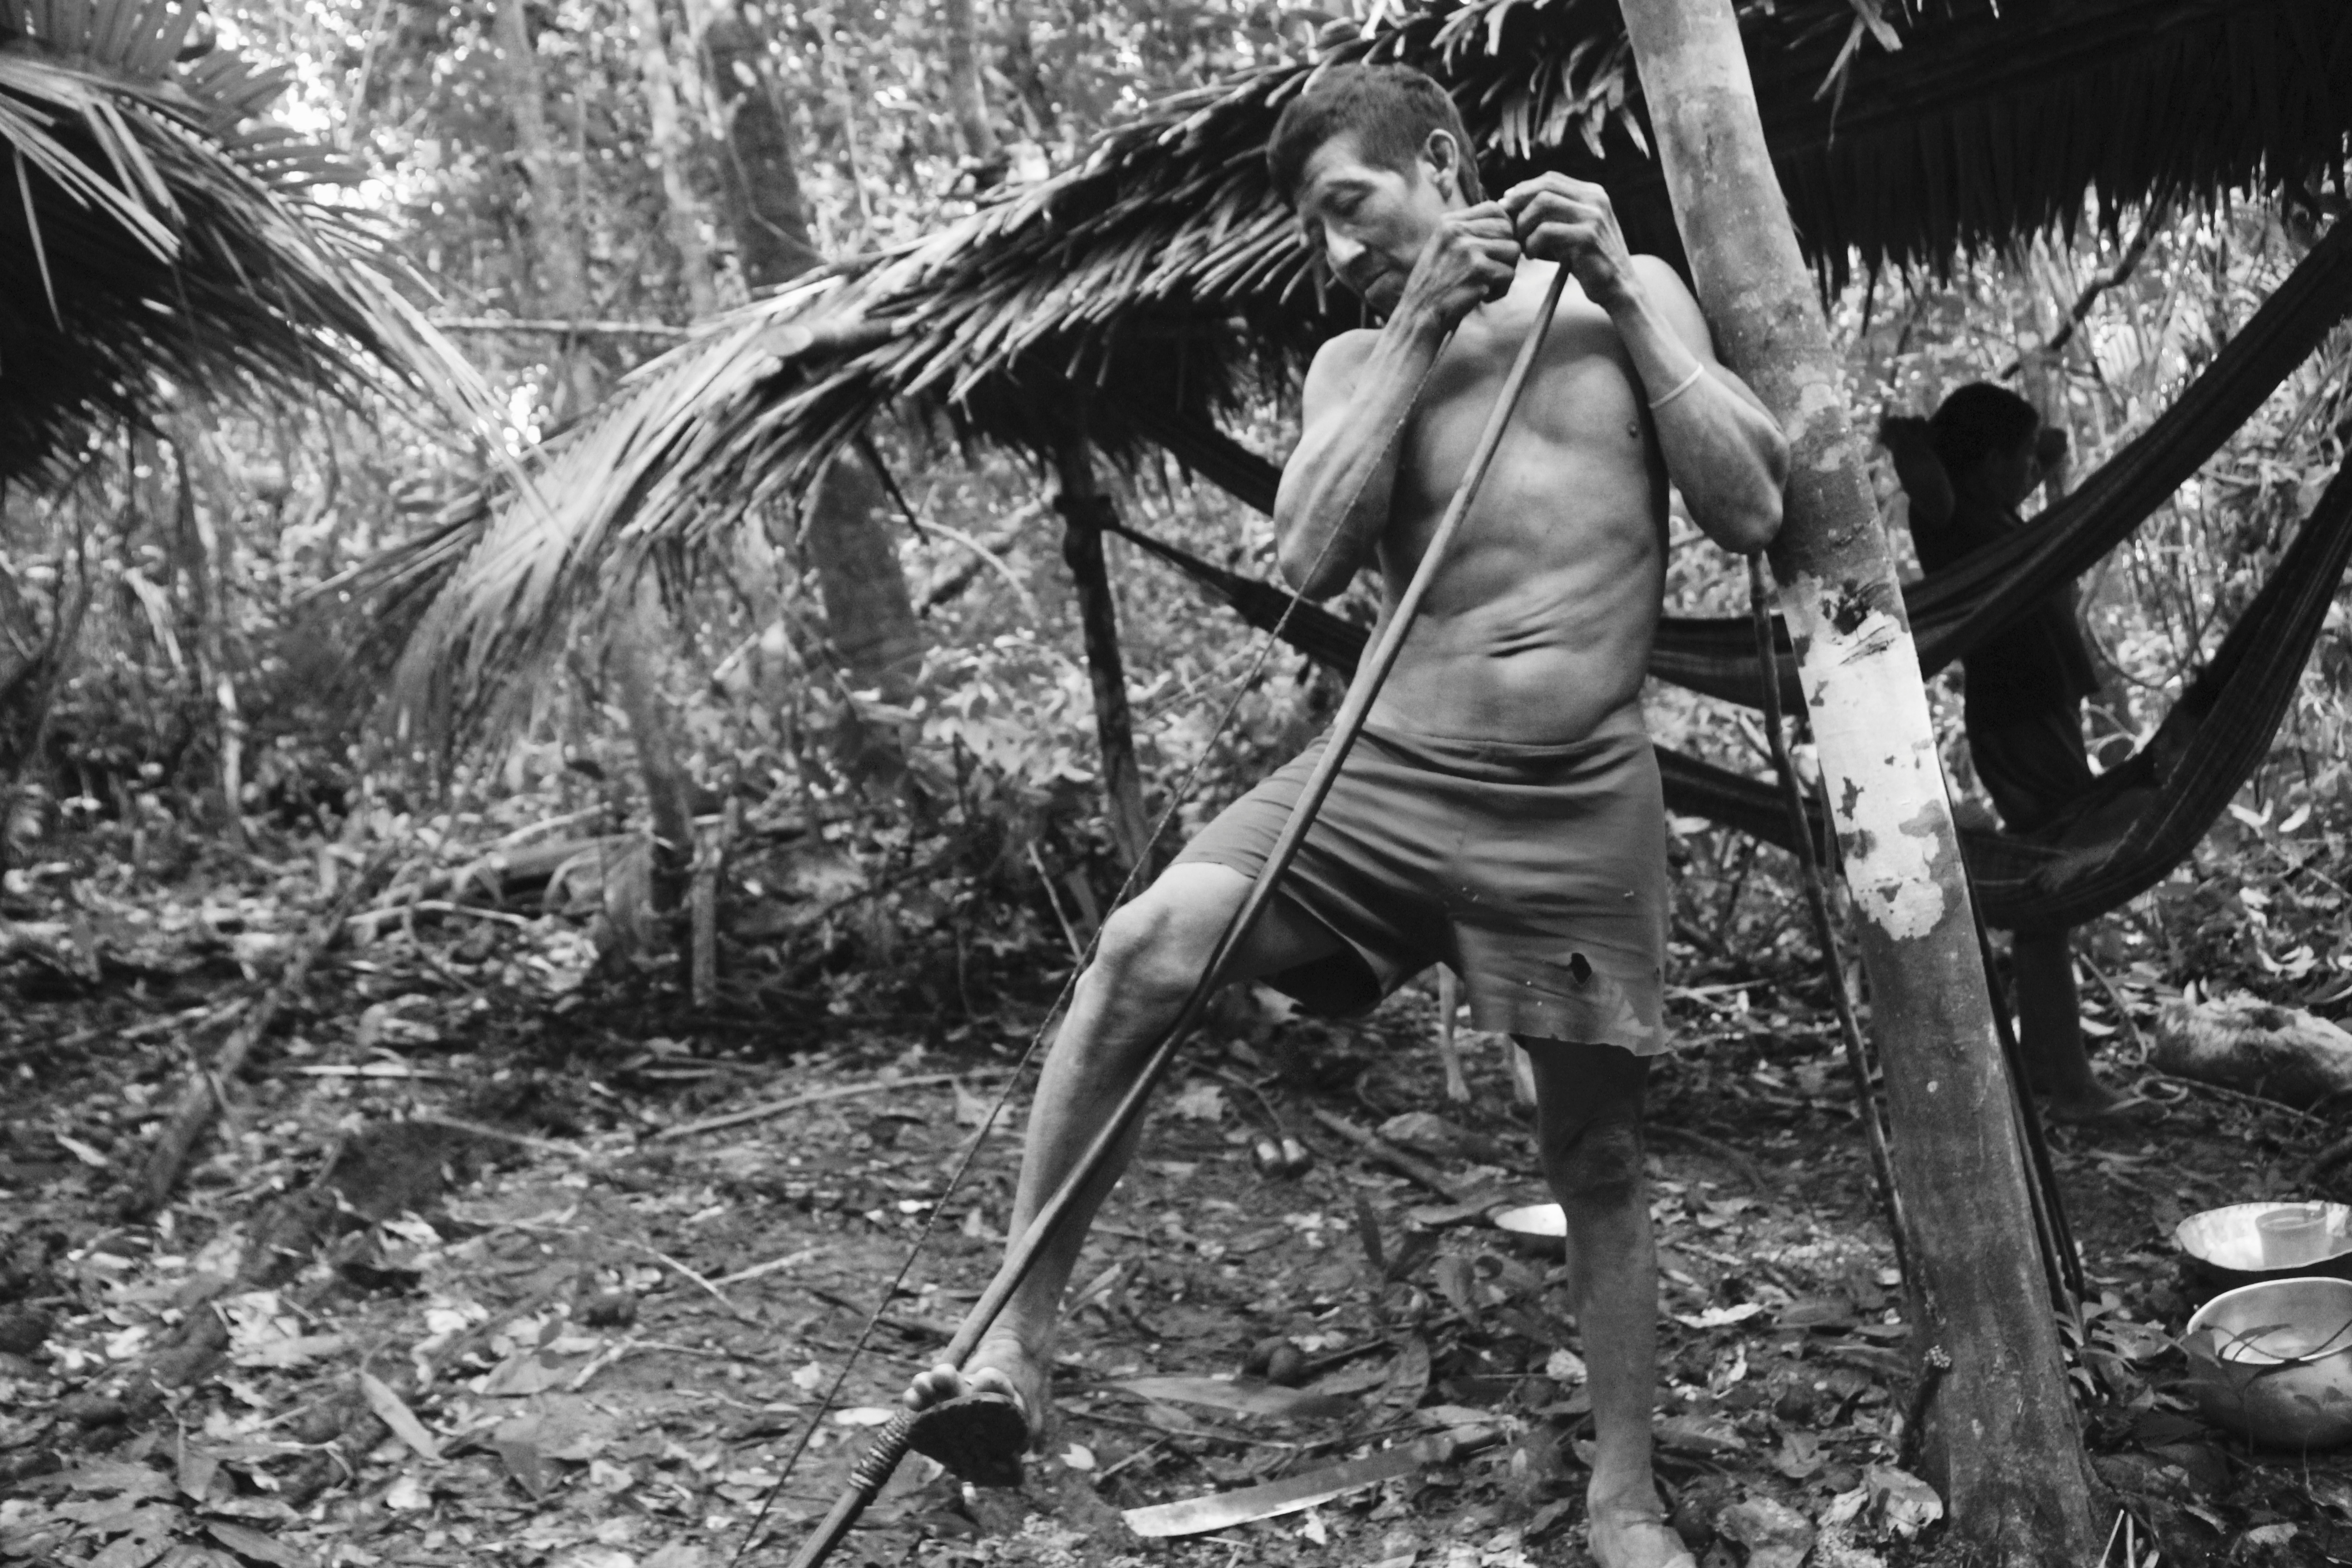
\includegraphics[width=\textwidth]{./imgs/IMG_1669}
\caption{Takamỹxa'a e seu arco. Ao fundo, na penumbra, sua esposa Irakatỹa descansa no tapiri (acampamento de caça, aldeia Tiracambu, 2013).}
\end{figure}

Ao sair de suas casas no final da tarde, além de estarem limpos, os
homens levam consigo uma rede (e as cordas para amarrá"-la), facas,
espingardas e alguma farinha. Quase sempre dormem à tarde para poder
passar a noite em vigília. Levam também algum pano para se proteger do
frio noturno. Tudo isso, bem amarrado às costas, segue com o caçador até
o local da espera, em alguma das árvores já mencionadas.. Estando lá,
nada na paisagem pode ser modificado; não se pode tirar uma folha de
lugar. A floresta deve ficar o mais intocada possível. O caçador deve
caminhar de leve pelo local para que as folhas não sejam espalhadas, as
pegadas não marquem o chão e o mínimo de galhos secos seja quebrado. Uma
vez escolhida a árvore para a espera, o homem amarrará sua rede no alto
da árvore entre dois troncos firmes --- subindo com a ajuda de caibros
amarrados, tal qual um sistema de andaimes ---, de modo que fique a uma
altura de uns cinco metros do chão, o suficiente para, aliado à
escuridão e ao silêncio, se camuflar. À noite, a floresta é repleta de
sons, e durante a espera noturna o caçador precisa estar com os ouvidos
bem atentos, pois junto com os passos dos animais ouvirá também o grave
som do sapo \emph{kapokapo}; o canto de cigarras e outros insetos; as
folhas remexidas por macacos"-da"-noite (\emph{aparikya}) e juparás
(\emph{haipaxĩa}). Ratos, gambás e outras criaturas da noite soltam seus
gritos; o barulho do vento nas folhas das árvores também sonoriza o
ambiente; além dos fantasmas \emph{ajỹ}, que circulam por boa parte da
floresta escura com seus assobios e batidas secas com pedaços de pau nas
árvores.

A espera (\emph{matakwa}) envolve um estado de completa atenção, que
pode ser expresso por termos como \emph{xa} \emph{katy} (``olhar bem''),
\emph{juanũ} (``ouvir"-atentar''), e \emph{jamaka} (que traduzo por
``prestar atenção'').

E, em que consistiria uma \emph{espera} (\emph{matakwa}) bem sucedida?
Para responder essa questão, listo abaixo os procedimentos e cuidados a
serem tomados durante a \emph{espera} \emph{matakwa} que --- mesmo não
garantindo o sucesso na caça --- são indispensáveis ao bom caçador.

\begin{enumerate}
\def\labelenumi{\arabic{enumi}.}
\item
\begin{quote}
  \emph{Não se deve sair de casa suado, sujo, nem exalando qualquer odor, pois
    os animais sabem pelo cheiro (\emph{kaxỹ}) que há um humano à espreita
    e fogem. O ideal é tomar um banho de rio antes, porém sabão, sabonete,
    desodorante ou outros produtos cheirosos dos brancos (\emph{karaia})
    não devem ser manipulados. Da mesma forma, estão vetadas as
    folhas"-remédios (\emph{pohỹ}) extraídas da floresta e que são
    utilizadas no tratamento de dores e doenças do corpo, já que seus
    odores também espantam as presas}.
    \end{quote}
\item
\begin{quote}
  \emph{Não se deve pisar em nenhuma fruta, folha ou galho depositado ao pé da
    árvore onde ocorrerá a espera, sob o risco de o animal que lá chegar
    perceber o rastro humano. Por isso deve"-se caminhar sempre descalço.
    Os chinelos de dedo devem ser mantidos em casa ou na sacola
    (\emph{marakũa})}.
    \end{quote}
\item
\begin{quote}
  \emph{Considerando"-se que o caçador precisará construir um andaime para se
    \emph{apoiar} e amarrar sua rede com tranquilidade na árvore, os
    caibros de madeira a serem utilizados devem ser retirados alguns
    metros antes do local da espera, já que nenhum barulho deve ser feito
    no entorno da árvore. Além do mais, não poderá haver mudança na
    paisagem. Esses caibros são amarrados entre duas árvores próximas, de
    modo a formar uma estrutura de três ou quatro níveis que possa dar
    acesso a uma altura de cerca de cinco metros do chão. Lá se amarrará a
    rede (a rede será amarrada nessas mesmas duas árvores onde se fez o
    andaime)}.
    \end{quote}
\item
\begin{quote}
  \emph{Uma vez o caçador instalado na rede, todos os movimentos devem ser
    executados de forma delicada e silenciosa, pois qualquer ruído pode
    espantar a caça; seja um leve mexer na sacolinha de munição ou um
    \emph{clique} produzido pelo engatilhar do cão da espingarda}.
    \end{quote}
\item
\begin{quote}
  \emph{A lanterna --- ferramenta de grande valia na espera noturna --- permanece
    amarrada à rede para ser sacada na chegada do animal. Ela é acesa
    instantes antes do tiro, apenas para o caçador encontrar a posição da
    presa com precisão. O tempo de iluminar a presa é o mesmo em que o
    animal percebe que está sendo observado e foge. Os Guajá lembram que
    ao ``jogarem luz'' na presa, antes da fuga (principalmente a anta, o
    veado e a paca), ela mantém"-se paralisada por poucos milésimos,
    olhando a fonte de luz. É durante esse tempo que devem atirar}.
    \end{quote}
\item
\begin{quote}
  \emph{Dormir está fora de cogitação.}
  \end{quote}
\end{enumerate}

Um dos maiores riscos envolvidos nas esperas noturnas é o encontro com
os \emph{ajỹ}. Muitas vezes o \emph{matakwa} (``espera)'' é mal
sucedido, pois os \emph{ajỹ} conseguem dispersar a caça. Os caçadores
contam que muitas vezes os animais são dissuadidos pelos \emph{ajỹ} de
tomarem certa direção para que não morram. Os \emph{ajỹ} espantam seus
animais, dizendo: ``não vão comer naquelas árvores, pois os \emph{karaia}
(não indígenas) estarão lá esperando vocês, eles estão escondidos e vão
matá"-los''. \emph{Karaia}, nesse caso, pode ser uma das formas como os
\emph{ajỹ} enxergam os caçadores humanos, devido ao potencial assassino
representado, principalmente, pela espingarda; além do fato de os
humanos, do ponto de vista dos \emph{ajỹ}, encarnarem a
\emph{diferença}, a ``diferença pura'' (ver AmaZone, 2010), uma pura
diferença inimiga.

Em um caso semelhante, ``donos dos animais'' e ``inimigos'' é a forma pela
qual os Araweté pensam os \emph{Ãñĩ}, que, tal como os \emph{ajỹ}, podem
ser definidos como o ``espectro terrestre do morto'' (Viveiros de Castro,
1986, pp. 216--217). Para os \emph{Ãñĩ} Araweté, os humanos são percebidos
como queixadas. Tal como para os \emph{ajỹ} Guajá, os humanos seriam não
indígenas e/ou inimigos. Para os \emph{ajỹ}, os humanos podem ser tanto
parentes distantes com os quais querem manter relações quanto, como
vimos acima, inimigos (não indígenas, ``índios brabos'', dentre outros).
As duas interpretações aparecem quando os Guajá falam dos \emph{ajỹ}.
Ora deve"-se manter distância, pois eles querem levar os humanos para
viver com eles; ora porque querem matá"-los. A posição de diferença
inimiga (expressa não só pela ideia de \emph{mihua}, mas também de
\emph{karaia}) entre os humanos e os \emph{ajỹ}, no entanto, aparece de
forma bastante nítida quando observada a partir das atividades de caça.
Caso um animal seja alvejado por um caçador e ainda consiga fugir com
vida, são os \emph{ajỹ} que cuidam de suas feridas e os advertem a terem
mais cuidado com os humanos. Como já coloquei anteriormente, os
\emph{ajỹ} mantêm controle sobre algumas espécies de animais de caça
(principalmente os veados, as pacas e os quatis), e são considerados
\emph{jara} desses animais específicos. Como também já discuti, a ideia
de ``dono dos animais'' (pais ou mães da caça, etc.) não apresenta grande
rendimento no caso Guajá, porém não significa que ela não opere
determinadas relações, tal como a dos \emph{ajỹ} com as pacas, veados,
quatis, gambás/mucuras (talvez, seu principal avatar, pois também são
chamados \emph{ajỹ}), macacos"-da"-noite, além de pássaros como o acauã.

O fato de a paca e o veado se alimentarem à noite também está
relacionado à ``proteção'' (\emph{riku}) dos \emph{ajỹ} sobre esses
animais, pois a floresta durante a noite (\emph{pyha}, ``noite''; ou
\emph{matarahỹ}, ``escuro'') é mais segura para esses animais. Por
exemplo, Pira'ima'ã me relatou que, certa noite, esteve frente a frente
com uma paca, mas que sua espingarda ``bateu'' (\emph{pehẽ}, ``quebrar'') e
não atirou. Em três tentativas de tiro, a espingarda ``bateu'', dando
tempo suficiente para que a paca fugisse. Pouco tempo depois, Pira'ima'ã
disse ter ouvido de sua rede (na espera) assobios e barulhos de
pauladas, o que indicava a proximidade dos \emph{ajỹ}. O caçador ficou
quieto, sentindo em seguida um arrepio por todo o corpo, seguido de
calafrios\ldots{} era este o sinal da proximidade dos espectros \emph{ajỹ}.

Se hoje toda espera noturna é realizada com espingardas, só conseguirão
realizar essa caçada os homens que manejam essa arma. Os mais velhos,
cuja arma de caça é exclusivamente o arco e flecha, nunca realizam
esperas, embora de alguma forma participem, indicando os bons locais de
caça e dando outras dicas sobre os animais. Ainda assim, as caçadas
noturnas (\emph{wata} \emph{matarahỹ} --- ``andar no escuro'') eram
realizadas antes do contato, embora se configurassem mais ativamente
como caçadas terrestres e emboscadas de animais. Naquele tempo, sem
lanternas e espingardas, a possibilidade de esperar um animal com chance
de acertá"-lo era muito menor do que hoje. Tochas e lamparinas, feitas a
partir de resinas (principalmente) da maçaranduba (\emph{mixiranỹkaha}),
jatobá (\emph{itawa}), jutaí (\emph{itai ihikira}) e amescla
(\emph{jawarakua}) sempre foram utilizadas como luz (\emph{hawa})
noturna para iluminar os caminhos (\emph{hape}, ``meu caminho''), nos anos
em que viviam na floresta (caçando ou mesmo fugindo). Ainda assim,
conseguem se locomover à noite sem fonte de luz com bastante
competência.

Em uma conversa com Wirahoa, ele me relatou que nasceu e cresceu fugindo
dos \emph{Tenetehara}; que seu pai morreu quando ele ainda era pequeno;
e que sua mãe lhe contava muitas histórias sobre morte entre os Guajá e
sobre a necessidade de seguirem fugindo dos inimigos \emph{kamara} e (os
não menos inimigos) \emph{karaia}. Para tanto necessitavam fugir pelo
escuro da floresta sem carregar qualquer fonte de luz --- somente um tição
em brasa (\emph{ira} \emph{tata}, ``pau de fogo'') para acender fogueiras.
Além de estratégia de sobrevivência, a caça noturna antes do contato só
era possível devido à capacidade que os homens têm de se locomover à
noite, sem luz. Essa capacidade é colocada em prática até hoje, durante
a espera noturna. Nas ``esperas'', muitos animais são alvejados, porém
alguns conseguem escapar, ainda que feridos. Caso percebam a proximidade
de um caçador por causa de sua lanterna, fugirão ainda que esgotem todas
suas forças nessa tarefa. Por isso, até hoje os animais são rastreados
no escuro da mata. Por exemplo, em agosto de 2009, Hajmakoma'ã matou sua
primeira anta. O tiro que ele desferiu não a matou prontamente. Ele teve
de segui"-la pelo escuro para capturá"-la. Mas mesmo portando uma lanterna
teve de mantê"-la desligada, uma vez que a luz poderia pôr a perseguição
a perder. Hajmakoma'ã explicou"-me que se o animal enxerga a luz e, mesmo
que esteja prestes a morrer, correrá até seu limite. Mas se não
pressente a presença humana, para e descansa. É nessa hora que será
morto pelo caçador, que estará invisível na escuridão.

\subsection{Outras esperas}

\forceindent
Além das esperas noturnas em que são utilizadas redes e lanternas,
pequenas esperas em beiradões e igarapés, que também envolvem silêncio e
atenção, são bastante realizadas, principalmente pelos mais jovens que
estão se iniciando nas artes da caça. Estas costumam ocorrer próximas à
aldeia e não exigem que o caçador passe uma noite inteira na mata --- o
que exigiria disciplina e força, que os mais jovens (e muitas vezes até
os adultos) não querem ter\footnote{Lembro"-me de alguns bons caçadores
  da aldeia recriminarem Pinawaxa'a pelo fato de ser um caçador
  incompetente, pois dormia durante a espera e ainda mantinha relações
  sexuais com a esposa, mesmo estando sem sorte na caça (\emph{panemuhũ}
  ``panema'').}. Essa espera ocasional pode ser representada pela palavra
\emph{juanũ}, que traduzo por ``atentar'' (sendo que -\emph{nũ} é
``ouvir/escutar''), e requer outros sentidos além da visão --- como a
audição --- como garantia de sucesso na caça. Como muitos animais vão à
noite para a beira do rio beber água --- como a paca e o veado, ou o
jacaré, que lá vive, e mesmo os tatus que vão ``caçar'' minhocas ---, essas
breves caçadas noturnas costumam deixar muito felizes os jovens de 15
anos (que já são hábeis no manejo de uma espingarda). O mais importante
é que consigam caçar no escuro.

Outra forma de ``espera'' bastante utilizada e hoje adotada com algum
entusiasmo é o chamado \emph{badogue}. Um misto de atiradeira e
armadilha --- muito utilizadas pelos moradores que vivem no entorno da
área indígena --- que foi propagado entre os Guajá por eles e funcionários
da \versal{FUNAI}. Desde essas poucas décadas de contato, alguns homens já
tiveram duas ou três espingardas pois, devido à utilização intensa da
arma, seu tempo de vida é muito menor do que prevê o fabricante. Chuva,
umidade, lama, quedas, além do feitiço dos animais contra esses objetos,
vários são os fatores que fazem as espingardas se quebrar, muitas vezes
sem chance de conserto. Quase sempre sobra a caixa com o gatilho e o
cão, além do cano, pois a coronha, base do cano e parafusos se perdem
quase que por completo. Quando é possível, os caçadores, com a ajuda de
funcionários da \versal{FUNAI}, esculpem novas coronhas, introduzem novas peças e
as adaptam ao antigo cano. Porém, outras vezes os canos ficam sem
utilidade e são readaptados e utilizados na confecção dos badogues ---
arma de caça que consiste em uma estrutura de madeira talhada, na forma
de uma coronha de espingarda, em que é adaptado um cano de espingarda
fora de uso. No corpo da madeira fazem uma câmara conectada ao cano,
onde será colocado o cartucho, e o disparo é feito por um forte tubo de
borracha cirúrgica --- o mesmo utilizado nas atiradeiras de crianças (ou
badogues, bodoques, dentre outros nomes) que conhecemos --- que aciona um
prego cuja ponta, ao bater na espoleta do cartucho, provoca o tiro. Os
badogues são colocados em locais onde se encontram rastros de animal e
servem fundamentalmente para matar pacas (\emph{kararuhua}). Um cabo
(uma linha grossa, ou mesmo fibra de tucum) é esticado de modo a
produzir o disparo assim que é rompido pelo animal, ao passar em frente
ao badogue. Essas armas costumam dar bons resultados, ao mesmo tempo que
(muitas) outras vezes falham, seja por falta de força da borracha ou
porque a espoleta, mesmo provocada, não dispara; ou até pelo fato de o
tiro ser dado, mas não atingir o animal, que estaria fora de alvo.

Outra forma de ``espera'' é a caça de tocaia (\emph{takaja}), que consiste
em uma espera diurna, em que o caçador fica protegido por uma estrutura
de folhas e não é visto pelos animais. A \emph{takaja} é um abrigo de
floresta, formado por uma estrutura de troncos fincados ao chão, de
forma circular, e envoltos por um grosso cipó que proporciona
sustentação às folhas de babaçu ou açaí que revestem o abrigo. O
principal objetivo do abrigo é ocultar totalmente o caçador em seu
interior, além de protegê"-lo de eventuais ataques de animais, por isso é
totalmente revestida, do chão ao teto, e seu interior, completamente
escuro. A pouca luz e o ar que recebe provêm de aberturas laterais muito
pequenas, imperceptíveis externamente, e que auxiliam na visão. Ao
passar perto desse amontoado de folhas, os animais não desconfiam da
armadilha e são surpreendidos por um tiro ou flecha. Adultos e crianças
armam \emph{takaja}, sendo esta, inclusive, uma das formas com que um
jovem se inicia nas caçadas. Meninos ainda muito jovens, entre oito e 10
anos, armam pequenas \emph{takaja} na floresta, próximo à aldeia, e com
auxílio de suas pequenas flechas e atiradeiras conseguem abater
inhambus, mutuns"-cavalos, jacus, jacamins, juritis e até mesmo pequenos
mamíferos, como o quati"-puru (\emph{tamakaja}) e a cotia
(\emph{akwixia}).

Uma \emph{takaja} pode ser construída tanto no solo (para a caça de
animais terrestres) quanto no alto das árvores, quando o objetivo é
caçar pássaros que se abrigam nas copas, como o tucano"-de"-bico"-preto
(\emph{takỹna}), específico da região, e o araçari (\emph{takyynihĩ},
``tucaninho''), aves importantes cujas penas são matéria"-prima para a
confecção dos diademas e braceletes utilizados pelos homens. As
\emph{takaja} feitas no alto das árvores podem ser montadas a grandes
alturas, de até 20 metros. A que vemos na foto foi feita por um caçador
experiente com a ajuda de seu cunhado. O homem subiu na árvore
carregando cipós --- um, inclusive, bem longo que, lá de cima, alcançava o
chão. Uma vez no alto, lançava o longo cipó para Juxa'a que o amarrou a
finos troncos de árvores (seis troncos foram necessários), depois folhas
da palmeira açaí e mais cipós, em várias subidas e descidas, tal como um
elevador de cargas. Em menos de uma hora, a \emph{takaja} estava pronta
lá no alto.

%(\textbf{foto da tocaia})
\begin{figure}[H]
\centering
  \includegraphics[width=\textwidth]{./imgs/IMG_1615}
\caption{Auxiliado por seu cão, Maihuxa’a caça uma cotia no buraco (acampamento de caça, aldeia Tiracambu, 2013).}
\end{figure}

\section{Palavras noturnas }\label{palavras-noturnas}

Não poderia deixar de mencionar aqui as palavras noturnas que, ao final
de um dia, consagram não só as caçadas, mas toda a vida. É à noite que
as pessoas comentam sobre os acontecimentos do Posto Indígena; sobre a
atitude de determinados funcionários; a preocupação com os invasores da
área; e tomam decisões que levarão aos funcionários da \versal{FUNAI} sobre
determinado tema, tal como uma ``política noturna'' (nas palavras Peter
Gow), que deve ser realizada cotidianamente. Além dos assuntos
cotidianos, minha presença na comunidade alterava o teor das conversas,
quando me sabatinavam sobre o mundo dos \emph{karaia} com perguntas,
como: se eu conhecia o então presidente Lula ou a liderança indígena
Marcos Terena; se em São Paulo havia Guajajaras; se meu sogro não se
zangaria por eu deixar minha esposa e filha sozinhas por tanto tempo; e
mesmo se eu não estava pensando em me casar com alguma mulher da aldeia;
--- dentre tantas outras questões que eu respondia, buscando compensar
minhas interpelações diárias e invasivas. Tudo ocorria sob o olhar
atento das crianças, a desconfiança dos velhos e o vigor dos jovens ao
perguntar, explicar, e tornar a perguntar. Além das caçadas, o tema que
mais causa comoção nas conversas noturnas são os invasores da área, cujo
impacto na vida das pessoas é óbvio. Os Guajá planejam ataques, ameaçam,
puxam arcos e marretas enquanto falam, prontos a matar um inimigo que
parece estar ao lado do narrador. Caça e guerra aparecem nas conversas
noturnas. E as noites sempre eram mais animadas graças a essas
narrativas.

Desde a volta do mato, quando chegam na aldeia, comentários e
brincadeiras já começam a ilustrar aquele dia de caçada. Há um tipo de
comentário bem"-humorado feito quando alguém retorna, quase sempre
proferido por outro que, em um primeiro momento não se beneficiará da
comida, muito provavelmente um afim distante, assim: ``Ah, você trouxe
caça para mim meu irmão/filho (\emph{haxa'a}), hoje eu vou comer
muito bem meu irmão''. Muitas gargalhadas são dadas, pois a caça em
questão não é para a pessoa que comentou, tampouco ela tem esse grau de
parentesco com o caçador. São piadas como essas ou cantos sobre
determinado \emph{karawara} (caçadores) que marcam a chegada das pessoas
nas aldeias. Porém, é à noite que as caçadas cotidianas são lembradas, e
por vezes toda a assembleia de uma aldeia estava atenta a uma única
pessoa, que contava os feitos do dia como se narrasse belos mitos. Essas
falas podem ser chamadas \emph{muumu'ũ} (``narrativas'') ou, como outras
conversas cotidianas, ``falas'', \emph{ma'iha}. Uma das experiências
estéticas mais fascinantes durante meu trabalho de campo foi poder ouvir
pessoas narrando e comentando caçadas, em um ritmo pausado, marcado por
silêncios e cadências que ressaltavam as situações, além de onomatopeias
e imitações magistrais, tal como ``imagens de sons'' (Kohn, 2013, p. 36).
Descola observa, para o caso Ashuar, que ``graças às intermináveis
histórias de caça que os homens gostam de contar, todo mundo também sabe
qual foi o comportamento do animal antes de morrer: o medo, a tentativa
de fuga abortada, o sofrimento, as manifestações de aflição dos seus
companheiros. Em suma, ninguém pode ignorar de que maneira um ser vivo
se torna comida'' (Descola, 1998, p. 29). Entre os Guajá, não só os
homens narram caçadas, mas é muito comum as mulheres serem ouvidas por
todos, quando complementam seus maridos ou mesmo protagonizam, por falas
exclusivas, seus feitos na mata. Os relatos (\emph{ma'iiha} --- ``fala'')
sobre as caçadas são ilustrados por imitações de sons de animais,
batidas e movimentos de mãos e pés. A mesma capacidade que os Guajá têm
para imitar os animais visando à predação é aqui utilizada para ilustrar
realisticamente a experiência do caçador. Essas narrativas não seriam
exclusivamente sobre ``caçadas'', mas remetem a uma experiência total, com
referência à extração de mel, passagem por antigos acampamentos, ataques
de \emph{ajỹ}, dentre outros eventos --- tudo o que estiver relacionado ao
\emph{wataha}, à ``caminhada''.

À noite, e mesmo durante alguns dias seguidos, um caçador pode se reunir
com outros e contar suas proezas: vangloriar"-se de como enganou uma
paca; comentar sua paciência durante a espera de um veado; a boa
estratégia na emboscada a um bando de capelães; a forma como o vento
dificultou sua audição durante a perseguição a uma ave; a resistência a
mordidas de muriçocas em uma noite quando esperava uma anta em um pé de
pequi; a alegria de saber que o jacaré que mergulhou, após ser ferido de
raspão, emergiu morto à superfície; o encontro com os \emph{ajỹ} durante
uma espera noturna, quando o caçador na madrugada fria soube manter a
calma e não se apavorar, esperando os espectros se dissiparem,
demonstração de grande coragem e sabedoria; a mordida de uma valente
cotia que se escondeu no fundo de um buraco já devastado (mas lá
resistia), e de como, mesmo ferido, o caçador aguentou a dor da mordida,
agarrou"-a pelo pescoço e conseguiu asfixiá-la; a flecha certeira, o tiro
perdido, a pólvora molhada\ldots{} tudo é lembrado à noite, à meia"-luz, sob o
embalo de comentários atentos, risonhos e curiosos.

Estes e outros acontecimentos --- ora insignificantes, ora fantásticos ---
compõem a vida de um caçador. Seus momentos de embate, no entanto, não
devem ser lembrados com remorso nem tristeza, ao contrário, com orgulho
e regozijo. ``Eu sou melhor do que uma onça, não tenho medo dela'',
disse"-me certa vez Pira'ima'ã depois de, orgulhoso, me mostrar dois
caninos de uma onça pintada que ele havia matado. ``Se ela tem unhas, eu
tenho a minha espingarda. Quando eu percebo uma onça no mato, eu a chamo
bem alto, `pode vir bicho, eu tenho uma espingarda e vou te matar!'" E
a onça, vista como bicho (\emph{hama'a} ``minha caça''), se torna menos
perigosa.

Ao iniciar minha pesquisa, não entendia de que se tratava aquelas
conversas tão compenetradas. Nada fazia sentido. Somente quando passei a
acompanhá"-los nas caçadas pude perceber que elas sempre eram remontadas
em fala, redramatizadas. Lembro"-me de uma específica vez em que
Hajmakoma'ã reproduziu o som de uma vara de porcos chegando ao longe,
sua boca ainda fechada foi se abrindo aos poucos, o que dava a real
sensação de que os animais estavam cada vez mais perto, se aproximando.
Em seguida, surgiram sons de folhas remexidas, dentes e rugidos. À
medida que ele narrava, novos sons apareciam, cada vez mais altos, até o
momento em que imitou o som de um tiro certeiro que mata um animal, e o
silêncio se restaura. É certo que eu não entendia nada daquelas
conversas, pois nessas horas os Guajá falam muito rápido e com a ajuda
de estalos, urros, gritos, assobios, como se a natureza do evento
penetrasse na palavra. Lima aponta o mesmo espanto ao descrever as
conversas Yudjá que antecedem uma caçada de porcos: ``em um instante já
não posso compreender o que os caçadores dizem. Todos falando ao mesmo
tempo, gritos estridentes, onomatopeias de explosões de tiros, flechas
silvando, porcos batendo os dentes, porcos em correria. Todos têm casos
para contar e mímicas para fazer'' (Lima, 1996, p. 22).

Ao ouvir sobre as caçadas, as pessoas ao redor muitas vezes parecem não
prestar atenção no que diz a boca do caçador. É comum o narrador parecer
estar falando com ninguém, todos mais preocupados em comer, descansar,
olhar para outro lado. Para participar da narrativa, as pessoas não têm
de estar necessariamente paradas, absortas pelas palavras, olhando o
narrador de forma fixa (dispositivo discursivo análogo ao de um chefe
ameríndio, cujas palavras nunca se transformam em voz de comando, tal
como sublinhou Pierre Clastres). Trata"-se de uma maneira de narrar, uma
forma de falar e ouvir os acontecimentos da vida que, no início (dado
meu despreparo etnográfico), cheguei a cogitar que fossem mitos, pois
todos (adultos e crianças) estavam muito envolvidos (embora parecessem
desatentos), juntos, como se aos mais jovens estivessem sendo narradas
fábulas fantásticas, de lugares outrora vistos apenas por poucos seres
no mundo e experiências que os humanos não mais conhecem. Mas os Guajá
não narram mitos, como narram caças. Preferem falar das caçadas e mesmo
de antigos eventos, a mitos. Discursos que versam sobre o desespero por
terem perdido uma trilha (\emph{pea}) e a alegria de reavê"-la; o choque
pelo encontro com uma onça ou fantasma e o alívio de retornar à casa,
com saúde e comida. Histórias por si só prodigiosas e que, devido às
formas poéticas, soavam ao etnógrafo como mitos. Os Guajá (e penso,
talvez, a maior parte dos povos ameríndios) não depositam na cosmologia
e na mitologia algo como um repertório narrativo que deve ser proferido
esporadicamente, como se isso salvaguardasse a \emph{sociedade} e fosse
uma transmissão de saber ou qualquer outra forma de \emph{socialização}
(nós, sim, fazemos isso!). O mundo (composto por viagens ao céu;
caçadores celestes; fantasmas na mata; relações sociais entre os
animais, dentre tantas outras características) é dessa forma, e não
precisam lembrar a ninguém que ele é assim. Aqui as pessoas não passam
seus dias falando sobre o céu e os mortos. Ao contrário, e ao menos para
os Guajá, o que faz de uma conversa algo interessante são os episódios
dramáticos da vida presente; que falem de comida ou do dia de caça que,
por si só, já são extraordinários.

A narrativa é contínua à caça, e está diretamente relacionada às formas
com que as pessoas atuam na floresta muito mais do que uma interpretação
isolada de uma ideia abstrata de caça e caçada. Ao contrário, relata"-se
uma caçada específica, e não uma idealização. Tal como observa Ingold
para as múltiplas produções de significado a respeito do espaço e
atividades nele envolvidas (Ingold, 2000, p. 56) --- e como já colocado
anteriormente --- em casos como o dos Guajá, separar a atividade de caça
de atividades como narrar as histórias e cantar seria tirar tais
narrativas que estão \emph{no} mundo (produzindo"-o, inclusive) e as
colocar como uma interpretação \emph{da} natureza --- algo que elas não
representam; tal como sua ideia de \emph{enskilment}, com que o autor
nos mostra o quanto fazer e aprender são processos inseparáveis para
muitos povos. No caso guajá, ao passo que todos riem e ficam apreensivos
com as narrativas de caça, também visualizam o tamanho do animal, a
configuração da paisagem, as decisões do caçador, dentre outras
informações que só aparecerão com a narrativa. As narrativas dos
caçadores Guajá enfatizam quanto suas presas se desesperaram ao vê"-los;
\emph{inimigos} (\emph{mihua}) que eram, ao mesmo tempo tais narrativas
consagram (lembrando os argumentos de Lima para a caça Yudjá) a
\emph{vitória da perspectiva dos humanos} (que prescrevem a caça) sobre
a perspectiva do animal caçado (que prescreve a guerra), pois o
contrário será sempre desastroso, como veremos agora. Tudo se passa como
se a caçada ainda não tivesse terminado. Aqui, ``a palavra é caça'' (Lima,
1996).

\section{\emph{Ha'aera e Panemuhũ}: ``Sobre isso não sabemos''}

A caça é uma atividade que envolve perigo, tanto em sua complexidade
técnica (já que é extremamente desgastante, com o caçador sujeito a ser
atacado por animais, machucar"-se de várias formas e mesmo falecer)
quanto pelo fato de muitos animais caçados serem dotados de
\emph{ha'aera} e, a partir disso, se vingarem dos humanos. O
\emph{ha'aera} é o mesmo princípio nocivo e raivoso que compõe a pessoa
Guajá (como vimos no capítulo 2) e que, após a morte, se transubstancia
no formato \emph{ajỹ}. No caso dos animais, o \emph{ha'aera} não se
transforma em \emph{ajỹ} --- isso só ocorre com o \emph{ha'aera} humano ---,
mas está próximo ao que a literatura etnológica sul"-americana denomina
como ``vingança'' (animal e/ou canibal) e termos congêneres (ver Lima,
1996; Hugh"-Jones, 1996; Viveiros de Castro, 2008). No que concerne à
caça, o \emph{ha'aera} pode ser lançado aos humanos por animais mortos,
pelos fantasmas \emph{ajỹ} e até mesmo por humanos mortos. Assim me
falou Wirahoa:

\begin{quote}
\emph{Quando vamos matar os capelães, eles ficam muito aflitos, pois pensam
que nós somos madeireiros. Após comermos sua carne, um deles vem durante
a noite, enquanto estou dormindo, e me diz: \emph{você me matou né, seu
madeireiro? Agora vou jogar minha raiva (ha'aera) em você}}.
\end{quote}

E, no dia seguinte, o homem pode acordar doente, com febre, indisposto.
Mesmo que goze de alguma saúde, pode experimentar um completo estado de
azar em sua vida. O \emph{ha'aera} pode atingir mulheres e crianças.
Nesse caso, quase sempre lhes causam doenças. Quando atinge e se aloja
nos homens, pode ser chamado \emph{panemuhũ} (termo que pode ser
traduzido por ``panema'').

Em um sentido lato, a ideia de \emph{panemuhũ} faz referência a um
conjunto de circunstâncias e estados que vão desde um mal"-estar --- como
uma indisposição, dores e cansaço excessivo ---, passam por doenças mais
graves e chegam até mesmo à perda do \emph{haitekera} (o princípio
vital). Uma vez \emph{panemuhũ} --- irritado, fracassado e sem paciência
---, o homem deve permanecer só em sua rede até que as coisas melhorem. Os
Guajá não gostam de conversar sobre o \emph{paneemuuhũ}, tal como fazem
com outros assuntos (como o \emph{iwa}, os animais, ou mundo dos não
indígenas). O assunto em si já deve ser evitado, e o mais comum quando
falávamos sobre o tema era eu ouvir ``É assim mesmo!'' ou ``Não sei não, eu
não lembro!'' ou ainda ``Pergunte para outro!'' Como se o fato de falar e
admitir o \emph{panemuhũ} fosse propiciá"-lo. Por isso, as informações
abaixo diferem de outras que constam neste trabalho; são fruto de pura
observação e interpretação, e não de conversas animadas e interessantes,
tais como as que mantive sobre outros temas\footnote{Algo muito parecido
  foi observado por Clastres em relação aos Guayaki. O autor informa que
  seus interlocutores tinham ``pouca prolixidade'' quando tratavam do
  \emph{pane}, termo cognato ao \emph{panemuhũ} Guajá: ``O que é
  \emph{pane}? Sob aparência anódina, essa pequena palavra perigosa
  designa de fato a pior das coisas que pode acontecer a um índio: a má
  sorte na caça'' (Clastres, 1995, p. 19)}.

Em sentido estrito, o \emph{panemuhũ} seria análogo à ideia de ``panema'',
o \emph{azar na caça} e outros infortúnios, tal como conhecido por
diversas comunidades tradicionais do Norte brasileiro (Galvão, 1976;
Matta, 1973; Wagley, 1988; e para um caso ameríndio, Clastres, 1995),
tendo sido discutido recentemente por Almeida (2007). Mesmo os Guajá
podem se referir a seus ``azares'' pelo termo \emph{panema}, em
``português'', tal como aprenderam com os \emph{karaia} nesses anos de
contato, que traduz de forma muito satisfatória o (termo cognato)
\emph{panemuhũ}. É muito comum um homem voltar calado da floresta e, ao
chegar em casa, comentar em português ``\emph{Tô panema}!'', como se
dissesse que a caçada foi improdutiva, ou mesmo como um sinal de que
algo pior havia acontecido. Mas, o que ocorre de fato nessas situações?
O que, além da morte, pode ocorrer de tão ruim a um caçador na floresta?

O estado \emph{panemuhũ} que acomete um caçador é, quase sempre, no
cotidiano o resultado de uma \emph{vingança} animal, isto é, uma
descarga de \emph{ha'aera} oriunda de algum animal abatido. Os
\emph{ajỹ} também, decerto, podem lançar o \emph{ha'aera} em um humano,
deixando"-o doente e/ou \emph{panemuhũ}. Veados, macacos, antas,
capelães, porcos, cotias, tatus, dentre outros animais, são dotados de
um \emph{ha'aera} violento. Desta forma, com uma formulação simples, o
\emph{panemuhũ} seria um estado circunstancial que um caçador (mas não
só um) experimenta após o ataque de um \emph{ha'aera}, seja ele
produzido pelos animais abatidos ou ex"-humanos \emph{ajỹ}.

Além disso, há um conjunto de atitudes e pequenos eventos que podem
produzir uma exclusiva má sorte na caça e que nem sempre está
relacionado ao potencial assassino do \emph{ha'aera}. Em outras
palavras, \emph{panemuhũ} pode ser tanto um sintoma grave de um ataque
espectral e assassino, relacionando"-se à saúde e composição de uma
pessoa, quanto um azar momentâneo resultado da quebra de uma regra ou
prescrição menor (algo como uma ``quebra tabu''). Existiriam, como em tudo
na vida, graus de azar\ldots{} e sorte, coragem, medo, alegria, tristeza\ldots{}
Da mesma forma, Clastres observa que o \emph{pane} entre os Guayaki era
evocado ``a propósito de circunstâncias ora graves, ora fúteis de sua
existência cotidiana'' (Clastres, 1995, p. 18).

Se um homem permanece durante sucessivas caçadas matando apenas pequenos
animais (tal como aves menores, tatus, roedores) ou mesmo capturando
apenas jabutis, ele deve se preocupar, pois pode estar \emph{panemuhũ},
uma vez que as grandes caças podem ter desaparecido. Assim, podem
provocar o \emph{panemuhũ}: 1. um acesso de raiva (ou a raiva contida);
2. tristeza ou aborrecimento de uma esposa em relação a seu marido; 3.
saudade e lembranças de alguém; 4. qualquer outro sentimento que altere
o humor do caçador ou de alguém para com o caçador, tornando"-o
``triste'', \emph{kije} --- notem que \emph{kije} é um termo cuja tradução
pode ser medo e/ou tristeza, sentimentos que neste contexto são
experimentados de maneira simultânea a partir da ideia de um
``medo"-tristeza''; 5. cócegas (\emph{kiinihĩ}) feitas por uma esposa ou
filhos nas axilas de seu marido/pai, pois ele perderia a firmeza no arco
ou na espingarda, seus braços ficariam ``moles'' e ele se tornaria
\emph{panemuhũ}; 6. caçar após o nascimento de um filho, pois esse pai,
além de não matar nada, pode enlouquecer; caso um homem vá caçar no
período de resguardo do nascimento do filho, um calor intenso se
apossará do seu corpo, um prenúncio da loucura; 7. em alguns casos (como
as caçadas de espera noturna), anunciar que está indo à mata pode causar
panem, pois os animais ``ouvem'' (\emph{nũ}) e, por isso, sabem
(\emph{kwaa}) que serão caçados; 8. alguns sonhos --- com cobras, por
exemplo --- também podem deixar o caçador sem sorte.

Além destas, há várias prescrições de ordem sexual e de atitude que
engrossam esta lista. Em linhas gerais, quando um homem está
\emph{panemuhũ} ele tem dificuldades de encontrar animais para caçar
(embora os animais não alterem seu ciclo), e é muito comum ele caminhar
durante todo um dia e não encontrar presa alguma; caso encontre, é bem
provável que não a mate. Os bichos simplesmente ``desaparecem''. É um
estado que, tal como uma doença, a pessoa que a contraiu sente. Nesses
casos, ele deve voltar para casa, falar com sua esposa o que está
havendo e descansar, pois quando o \emph{panemuhũ}/\emph{ha'aera} é de
um tipo fraco ele tende a passar.

Trata"-se aqui de ``um conceito altamente abstrato, como gravidade'',
como observa Almeida sobre a complexidade da ideia de ``panema'' entre
seringueiros do Acre --- uma ideia que envolve mecanismos e regras
particulares que, por sua vez, põem em relação uma ontologia diferente
da ``nossa ontologia naturalista que distingue domínios naturais e
domínios morais'', constituindo"-se uma ``economia ontológica da caça'':

\begin{quote}
\emph{(Panema) é um estado que é sentido no corpo, assim como sentimos um
peso; (\ldots{}) Panema, exatamente porque é tão generalizado como a
gravidade, e tão difuso como a honra pessoal, é algo que se confirma a
todo o momento pela experiência. Tudo se passa, de fato, como se panema
fosse parte do mundo. (Panema é um componente generalizado da
ontologia de caçadores da planície amazônica; e é confirmado"-corroborado
por encontros pragmáticos cotidianos. Para meu pai, que na infância
viveu na mata com meu avô seringueiro, e depois tornou"-se bancário de
carreira, assim como para o líder político e sindical Osmarino Amâncio,
panema nada tinha a ver com superstição, ou com religião, que ambos
rejeitavam por razões diversas. Panema era um fato do mundo, que a
experiência confirmava) (Almeida, 2007, pp. 08--09)}
\end{quote}

Um ``fato do mundo'', confirmado pela experiência, também me parece uma
excelente definição para o \emph{panemuhũ} awá-guajá, uma vez que tal
estado é sentido e experimentado por todos em um ou outro momento, em
diferentes situações de vida.

\section{Nem tudo é azar}

Embora me faltem elementos suficientes, gostaria de lembrar que, assim
como alguns eventos e fatores desestimulam uma boa caçada, outros podem
ajudar. Desta forma, alguns sonhos são propiciatórios, como sonhar com
onças; já que, segundo Pira'ima'ã, a onça é um grande predador, e vê"-la
em sonho pode ser sinal de que o caçador, ele mesmo, vá matar muitos
animais. Não sei se é uma regra geral, mas, ao menos para Pira'ima'ã,
sonhar com onças é um dos melhores prenúncios para uma boa caçada.

Muitas vezes os Guajá abatem fêmeas prenhas e, em todos os casos, os
fetos são consumidos como iguarias. Fetos de cotia, de capelães, além de
porcos e de antas são muito apreciados. No caso de quase todos os
grandes animais fêmeas em adiantado estágio de gestação (principalmente
antas, queixadas e caititus), as pessoas lavam a mão no líquido
amniótico da placenta, ao retirar o feto morto. No caso da anta, obtive
duas explicações pare esse procedimento: (1) que o líquido chamado
\emph{imymy} \emph{tekwera} (``líquido da criança dela'') ``educaria'' a mão
do caçador para que ele mate mais antas, (2) que ele fortaleceria o
corpo de quem lava as mãos, uma vez que o couro da anta é bem duro. Em
todo caso, me justificaram que lavam a mão no líquido amniótico de
outros animais como um procedimento propiciatório, e que isso atrairia
mais caça. Pode"-se lavar as mãos no líquido amniótico de diversos
animais, porém isso quase nunca ocorria quando matavam caças pequenas
(capelães, macacos, cotias). Era mesmo um ``procedimento propiciatório
ocasional'' (já que os Guajá, avessos a cerimônias, não praticam ritos de
caça ou caçadas rituais)\footnote{É importante enfatizar que, embora
  apreciem comer carne de ``vitelas'', os Guajá não têm predileção
  especial por matar fêmeas grávidas; ao contrário. Foi com pesar que,
  certa vez, Wirahoa recebeu a notícia de que a anta que seu irmão
  Hajmakoma'ã matara estava prenha e o filhote, prestes a nascer. O
  filhote já estava bem formado e até malhado, com são os filhotes de
  anta. Disseram"-me que, em casos como esse, retiram logo o filhote da
  mãe recém"-morta para os tomar como animal de criação. Como aquela foi
  a primeira anta que Hajmakoma'ã matou, ele não teria tido a habilidade
  necessária para salvar o filhote.}.

Em outra ocasião que também envolvia a caça de uma anta, após chegar ao
local onde Pira'ima'ã havia matado o animal horas antes, seu amigo
Pinawaxa'a deu alguns tiros no corpo do animal morto, gritando ``venha
anta, venha que eu vou matar você''. Pouco depois outro homem, Kamara,
chegou ao local e flechou por várias vezes a anta com uma taboca. Disse
que era para dar sangue para sua flecha e pela vontade (\emph{xaku'uhy},
``ver"-querer'') que também sentia de matar antas. De certa maneira, embora
estejamos falando sobre caça, isto remete a uma passagem de Descola
sobre a guerra Ashuar, quando diz que ``a morte de um inimigo é assunto
coletivo: assim que um membro do grupo dá o tiro mortal, todos
descarregam as espingardas sobre a vítima abatida e se tornam, por esse
ato, coassassinos solidários, de modo que os jovens ainda inexperientes
começam desde muito cedo a acumular façanhas'' (Descola, 2006, p. 346).
Talvez seja por isso que eu não mais me surpreendia quando chegava à
aldeia, voltando de uma caçada junto com determinado grupo (todos nós
carregando aves, macacos, pacas, cotias e, por vezes, quilos de carne
moqueada), e quem estava no pátio (e não havia estado na floresta) me
rodeava para ver o que eu trouxera, perguntando ``o que \emph{você}
matou, Uirá?'', embora eu não tivesse dado um tiro sequer; ou à noite,
quando estávamos comendo, me incluíam como responsável pela morte do
animal que estávamos consumindo. Nas caçadas de que eu participava,
mesmo não matando uma presa sequer, eu era tido como um responsável, com
se eu fosse --- parafraseando Descola --- um cocaçador solidário. No início
pensava tratar"-se de apenas um gesto de generosidade, do tipo ``nós
aceitamos você aqui!''; porém, aos poucos fui percebendo que assim
acontecia com outras pessoas. Por isso mesmo, talvez uma das maiores
indelicadezas que alguém possa cometer é se vangloriar de ser melhor
caçador do que outro; ou se vangloriar de feitos que, todos sabem, são
coletivos. Quando um homem vai mal na caça, não é por uma incapacidade
``natural'' como ``falta de talento'' --- tal como nós justificamos nossas
habilidades e a falta delas --- mas porque deve estar fazendo as coisas de
forma equivocada, já que se as fizer da maneira correta poderá ter
sucesso. Era assim com um finado amigo da aldeia juriti, considerado um
``mau caçador'' por muitos. Não que ele não soubesse caçar, ao contrário;
mas é porque ele quebrava diversas prescrições fundamentais ao bom
caçador --- por exemplo, mantinha relações sexuais de forma desmedida
(mesmo que à força) com muitas mulheres da aldeia e em seguida queria
caçar; mesmo estando doente, ia para a floresta; dormia na espera; não
cuidava bem de suas armas de caça --- muito mais do que seria um caçador
sem talento; para os Guajá, um ``mau caçador'' é aquele que não obedece as
regras do jogo.

\section{\emph{Ha'aera}, aqui tudo é azar}

Voltemos porém ao \emph{ha'aera} que, ao que tudo indica, é a principal
causa de \emph{panemuhũ}.

Um dos principais e mais devastadores efeitos do \emph{panemuhũ} é o
poder de desconectar a pessoa de seu princípio vital, de sua
``vitalidade'', o \emph{hajtekeera}. Uma clássica ``perda da alma'', em
termos xamânicos amazônicos, já foi bem discutida por alguns autores
(para um balanço, ver Viveiros de Castro, 2002, pp. 345--399). É esse mal que
a vingança dos animais (\emph{ha'aera}) e dos \emph{ajỹ} produz nos
seres humanos. Se pensarmos o \emph{panemuhũ} a partir da fisiologia da
pessoa, awá, da relação entre os elementos \emph{hajtekeera}
(``princípio vital''), \emph{ha'aera} (``raiva'') e \emph{ipirera}
(suporte físico, ``corpo"-pele''), veremos que pressupõe um
enfraquecimento, muitas vezes um abandono do \emph{hajtekera} (o
princípio vital), devido a algum trauma --- como um susto ou uma grande
dor --- sobre o \emph{ipirera} (o corpo), ou mesmo um elevado acúmulo de
\emph{ha'aera} (``raiva'') no corpo, provocado por mau"-humor
(\emph{imahy}, ``braveza'') ou tristeza (\emph{kije},
``medo"-tristeza''). Desta forma, um dos piores males a acometer um
caçador (e em consequência, sua família) é ele receber uma grande dose
de \emph{ha'aera} como vingança de uma presa abatida, capaz, inclusive,
de expulsar seu \emph{hajtekera} do corpo e deixar em troca o
\emph{panemuhũ}. Em linhas gerais, um homem se torna \emph{panemuhũ}
e/ou doente quando se distancia de seu princípio vital (seu
\emph{hajtekera}). Se imaginarmos o \emph{panemuhũ} a partir da
fisiologia da pessoa guajá --- da relação entre \emph{hajtekera}
(``princípio vital''), \emph{ha'aera} (``raiva'') e \emph{ipirera} (suporte
físico, ``corpo''), como vimos no capítulo 3 ---, os Guajá sugerem que o
\emph{panemuhũ} pressupõe um enfraquecimento e, muitas vezes, abandono
do \emph{hajtekera} devido a algum trauma no \emph{ipirera} (o corpo),
ou mesmo a um elevado acúmulo de \emph{ha'aera} no corpo (já que todos
têm uma taxa mínima de \emph{ha'aera}).

Como vimos no capítulo 3, os \emph{ajỹ} são puro \emph{ha'aera} --- quase
que de forma condensada. Esta é sua matéria autêntica, e eles a emitem a
um caçador, impossibilitando"-o de caçar. Em alguns casos, o
\emph{ha'aera} é provocado pelo fato de o homem ter passado por locais
frequentados por esses fantasmas, como um antigo acampamento, que pode
ser hoje a aldeia dos \emph{ajỹ}. Passar em lugares como esse é se expor
aos \emph{ajỹ}. Como já observei para os \emph{ajỹ}, a eficácia e
penetração do \emph{ha'aera}, emitido à noite pelos animais, são
comparadas ao grau de penetração que os odores e gases encerram. Por
isso explicaram"-me ser este princípio algo como o ``gás do meu lampião''
ou ``o aerosol de meu repelente'' --- algo invisível e espectral, porém
dotado de grande penetração. Em uma tradução geral, podemos afirmar que
o \emph{ha'aera} são agentes patogênicos, lançados aos humanos por algum
ser externo, como ataque ou vingança, e que causam doenças e morte.

Quem ataca os humanos é o próprio \emph{ha'aera} do animal, uma parte
dissociada da presa morta que se transforma em espectro. Ele é liberado
pela presa após sua morte e pode se instalar no corpo de qualquer um. De
acordo com a fala de Wirahoa que destaquei acima, o \emph{ha'aera} seria
uma parte do capelão --- por isso e ao mesmo tempo, ele próprio. No meio
da noite, o caçador e --- a depender da potência do golpe --- toda sua
família podem acordar doentes. Muitos animais encerram um \emph{ha'aera}
perigoso: capelão, paca, cotia, veado, anta. Após serem consumidos, seu
\emph{ha'aera} pode voltar à noite, à casa do caçador, e atacá"-lo. Se o
\emph{ha'aera} for suficientemente forte, pode se abater sobre mais
pessoas.

Além do \emph{ha'aera}, muitos animais teriam um \emph{haitekera} (um
princípio vital) que, em alguns casos e após sua morte, se encaminharia
para um determinado \emph{iwa} (``céu'') --- não exatamente o dos humanos ---,
enquanto seus \emph{ha'aera} permaneceriam na Terra para se vingar dos
humanos. Sobre o destino dos \emph{haitekera} das presas, como já disse,
as informações variam. Alguns disseram que existem céus específicos,
outros, que ascendem aos muitos \emph{iwa} dos humanos e lá passam a ter
uma existência diferenciada. Alguns preservam sua forma animal, porém
com a pele ligeiramente avermelhada (como muitos seres e coisas do
\emph{iwa} --- a água celeste vermelha e os capelães celestes vermelhos,
por exemplo). Outros se tornam humanos e vão viver em patamares
longínquos, onde os Guajá que visitam o \emph{iwá} nunca os conseguirão
alcançar.

\begin{center}
***
\end{center}

Wirahoa estava com um abcesso na testa, algo como uma grande espinha,
dura, inchada e que já lhe doía há meses. Sem querer espremer para
retirar o pus, estava tomando anti"-inflamatórios que lhe eram fornecidos
pelos auxiliares de enfermagem. Certo dia, relatou"-me que estava cansado
das dores em sua testa e decepcionado com os remédios dos \emph{karaia}
que, segundo ele, deveriam expulsar aquele ``chumbo de espingarda'' que se
alojara em sua testa e que lhe fora, meses antes, lançado por um tatu
que sobreviveu a um tiro seu. Ele contou que depois de avistar um tatu,
durante uma caminhada na mata, atirou no animal. Por causa de sua
carapaça, o tatu conseguiu fazer com que o chumbo do tiro retornasse na
direção de Wirahoa e se alojasse (exatamente) em sua testa (por isso ela
estava inchada daquele jeito) e em seus braços (por isso vinha errando
tantos tiros durantes suas caçadas). Com ajuda de Almir, um auxiliar de
enfermagem que à época trabalhava no posto, Wirahoa teve seu rosto
lancetado por um bisturi, o que liberou uma grande quantidade de sangue
e pus: ``venenos'' que estavam em seu corpo. Após limpar o ferimento, o
funcionário suturou com alguns pontos, e dias depois Wirahoa já estava
bem de novo. Inicialmente, Almir se recusou a drenar o abcesso de
Wirahoa porque, devido à grande inflamação, o exsudato poderia demorar a
sair, mas disse que com os remédios que lhe administrara o inchaço
desapareceria. Mas o homem insistiu com o auxiliar de enfermagem. Não se
conformava, pois sabia que o que estava em seu rosto era um pedacinho de
chumbo que o tatu lhe mandara de volta. Após esse episódio, me
explicaram que até animais de pequeno porte, como as cotias e os tatus,
podem apresentar perigo e jogar"-lhes \emph{ha'aera}. O perigo do tatu
está no seu ``couro duro'' (\emph{ipire} \emph{hatỹ}), segundo os Guajá.
Ele pode sobreviver aos tiros, além de fazer pedaços de chumbo voltarem
para o caçador e se alojarem de forma invisível em seus corpos. Por isso
mesmo, a carne de tatu é recomendada ao consumo quando alguém está com
cortes, luxações, entorses, dentre outros sofrimentos físicos que os
atingem a todo o tempo.

As espingardas, que apresentam muitos problemas, principalmente em suas
molas e parafusos; várias vezes são avariadas por forças invisíveis
contidas nos animais caçados --- muitas vezes chamadas \emph{ha'aera} (mas
também ``faquinhas'', ``flechinhas'', ``foguinho'', dentre outros nomes em
português). Por esse mesmo motivo, o poraquê (\emph{manakya}) é um
animal cuja caça não pode ser realizada com espingarda, somente com
flechas. O poraquê, por ter energia (\emph{tata}), emite uma descarga na
espingarda do caçador, fazendo"-a escangalhar"-se. Pira'ima'ã me relatou
que isso ocorreu diversas vezes, até perceberem que a energia do poraquê
atingia suas espingardas. É bom lembrar que, hoje em dia, os Guajá
preferem caçar qualquer animal com suas espingardas, mesmo pássaros
pequenos são pegos com esta arma e cartuchos que são recarregados,
muitas vezes, com excesso de pólvora e chumbo. Isso faz com que ele se
parta, além de destroçar partes do animal que seriam consumidas ou o
destruir quase por inteiro, como no caso de pequenos pássaros. É muito
comum encontrarmos pedaços de chumbo em meio a pedaços de carne enquanto
comemos. Matar os poraquês atirando"-lhes com espingarda era uma decisão
bastante aceitável, tendo"-se em vista o gosto dos Guajá por essa arma.

O cerco ao poraquê envolve absoluto silêncio e paciência. Horas antes de
chegar aos brejos e igapós, que habitam, deve"-se permanecer quieto,
pois, caso contrário, o peixe ``ouve'' as pessoas e foge. Em volta da
lagoa, o silêncio é absoluto. De quando em quando o poraquê emerge à
superfície e, rapidamente, volta a submergir. É em uma dessas subidas
que ele deve ser abatido. O animal é acompanhado pelo caçador, que fica
atento a seu movimento. Assim, o caçador deve prever quando e onde será
a próxima emersão. Juriximatỹa me contou que certa vez caçava com seu
cunhado em uma lagoa e conseguiram matar um poraquê, enquanto outro que
lá havia conseguiu escapar. Depois de voltar para casa, sua espingarda
subitamente parou de funcionar; estava ``batendo'', isto é, o cão estava
sem a força necessária para disparar a espoleta (algo que acontece com
frequência). Segundo Juriximatỹa, o poraquê que sobreviveu, durante sua
fuga, conseguiu jogar \emph{tata} (energia) em sua espingarda que,
então, ficou ``mole'' (\emph{myny}) --- \emph{manaky maka myny}: ``o poraquê
amoleceu a espingarda''. Gostaria de lembrar que antigamente
(\emph{imỹna}) não havia poraquês, até que \emph{Maira} jogou um de seus
arcos mágicos no rio e este se transformou em poraquê. O arco de
\emph{Maira}, tal como sua flechas, eram dotados de energia, por isso
ele era um grande caçador. E a mesma energia do arco de \emph{Maira} se
manteve no poraquê. Perigoso como um arco energizado, ele deve ser
caçado com muito cuidado. Por isso mesmo, hoje em dia, quase sempre na
estação seca, todo o poraquê consumido na aldeia Juriti é caçado por
homens velhos, que não manejam espingarda, mas que sabem que suas
flechas e arcos são imunes a esses ataques. Vemos que, além dos humanos,
seus objetos também podem receber o poder destruidor do \emph{ha'aera}
dos animais.

Se um homem vai à floresta desconfiado ou amedrontado, estará mais
suscetível a ataques de \emph{ha'aera} e à consequente perda do seu
\emph{hajtekera} --- caso extremo, porém, que atinge todo caçador e seu
equipamento de caça, que pode se tornar imprestável. Para melhor
apresentar esse tema gostaria de retomar de forma mais substancial um
caso que apresentei no capítulo 2, o do ataque por \emph{ajỹ} sofrido
pelo jovem Kaawi'ia. Para tanto, irei --- somente dessa vez --- reproduzir
um trecho de um de meus diários de campo:

\begin{quote}
\emph{Ontem Kaawi'ia foi mordido por uma espécie de lagarta que eu nunca
tinha visto e que chamam de ``rabo de veado'' (arapaha rawaraira), pois de
fato parece um rabo de veado. Outro nome que me deram para essa lagarta
foi ``formiga veado'' (arapaha taninĩa). Hajmakoma'ã, seu cunhado (\versal{MB}),
estava muito assustado e foi até a enfermaria, na sede do posto, junto
com o abatido Kaawi'ia que, além de uma aparência péssima, estava
assustado. O braço esquerdo de Kaawi'ia --- o mesmo braço que tomou a
picada --- estava muito inchado, e a auxiliar de enfermagem
administrou"-lhe um anti"-inflamatório e uma pomada. Desde ontem, quando
saiu da enfermaria, Kaawi'ia está em casa, na sua rede. Passou boa parte
do dia de hoje limpando sua espingarda e seus cartuchos (acho que, com
medo de que a doença lançada em seu corpo tenha se lançado também em seu
equipamento de caça). Hoje à noite, Panypinuhũa me disse que parte dos
relâmpagos no céu eram a hajtekera de Kaawi'ia cantando no céu, e que
estava com vontade de voltar para casa. Sua hajtekera fugiu devido à
dor, ao susto e ao medo pelos quais Kaawi'ia passou.}

\emph{Panypinuhũa disse: hajtekera jã wate!, a ``haitekera (dele) está
cantando lá no céu!'' por causa da doença de Kaawi'ia. Vim a saber que o
que ocorrera à Kaawi'ia fôra um ataque bem sucedido dos ajỹ, que deixou
o rapaz com tanto medo e dor que sua haitekera fugiu para o céu (wate ---
``longe para cima''). Ela se desvencilhou de seu corpo e lá permaneceu
cantando.}

\emph{Observando o episódio, tive a impressão de que um ataque de ajỹ
pode não só prejudicar o caçador atacado, como também suas flechas,
arcos e espingardas. Esses instrumentos, aliás, parecem ser tão
vulneráveis a ataques de ha'aera dos animais e fantasmas quanto o são os
humanos, e por isso os objetos também podem perder suas potências e
ficar ``azarados'', panema. Talvez por isso Kaawi'ia, mesmo doente pelo
ataque, em casa manteve"-se desmontando e limpando obsessivamente sua
espingarda, como se estivesse verificando, ou mesmo garantindo, que ela
não ficasse panemuhũ. (aldeia Juriti, 13/08/2009, caderno de campo nº
8)}
\end{quote}

Medo (\emph{kije'}) é uma palavra que definitivamente não pode figurar
no léxico de um caçador. Os animais devem ser abatidos sem remorso, e o
momento da morte das presas, mesmo que relembrado nas falas noturnas,
deve ser em seguida esquecido. Me explicaram que para que eu fosse um
bom caçador eu não poderia ter pena. Fica o feito heroico; porém as
preocupações, angústias e medos --- que todos podem sentir --- não devem ser
rememorados. Boa parte dos riscos de uma vingança animal são eliminados
quando o caçador simplesmente não se importa em matar suas presas ou
esquece as situações em que as mortes ocorreram. Por essas e outras, os
Guajá sempre gostam de lembrar que ``bicho não sente dor''. E caso as
lembranças negativas de caçadas sejam sistematicamente relembradas (como
o engasgue ou falha de uma espingarda; o corte profundo no pé; o
rompimento da corda do arco, ou qualquer outro evento desastroso), as
coisas podem ficar perigosas. Não que a lembrança em si crie o problema,
mas ela acentuará o que já está errado (os erros e azares que um homem
pode estar tendo). A frieza de um caçador é sua melhor arma. Por isso,
os jovens caçadores (como Kaawi'ia) são mais suscetíveis a ataques de
``almas'' (\emph{ajỹ}) e outros \emph{ha'aera}; e por vezes perdem o
controle ao voltar da aldeia (como já discutido). Esquecer a dor e o
momento da morte do animal é imprescindível. Esquecendo"-se do bicho, a
raiva (\emph{ha'aera}) dele não se aproxima --- ou tem menos chance de se
aproximar --- dos humanos.

Lembro"-me de nossas primeiras conversas sobre os \emph{ajỹ}, quando me
explicaram não haver seres assim nas florestas próximas à aldeia Juriti;
que os \emph{ajỹ} viviam próximos às outras aldeias dos Guajá. E o mesmo
era dito do \emph{ha'aera}. Muitas vezes diziam desconhecer o assunto.
Outras vezes, que os animais não lançam mais \emph{ha'aera}. Mas, às
vezes, escapava uma ou outra declaração que comprovava o perigo. É como
se os Guajá dissessem: ``Eu não acredito em vocês, vocês não me atingem,
pois não existem''. Dizem que quando uma paca é morta seu \emph{ha'aera}
fica no buraco onde ela vivia até ir embora. O mesmo ocorreria com os
tatus e cotias, cujos \emph{ha'aera} ficam no buraco; ou os capelães,
cujo \emph{ha'aera} permanece na copa da árvore. A lembrança
(\emph{imarakwa}) é sempre um componente perigoso. É assim com os
mortos, que devem ser esquecidos, e é assim também com os animais
abatidos que, mesmo depois de mortos, podem ser perigosos.

Vejamos mais dois episódios.

\subsection{\emph{Ha'aera} de anta}

\forceindent
Diferentemente de outros povos amazônicos, os Guajá não costumam caçar
de dentro de canoas. Como vimos, eles nunca navegaram, e seu território
ancestral era desprovido de grandes rios. No entanto, nos dias atuais a
geração jovem, principalmente, tem"-se utilizado de canoas --- que foram
incorporadas recentemente à vida social ---, para fazer esperas noturnas à
beira do rio e igarapés, a fim de caçar animais que porventura lá
apareçam. O episódio seguinte transcorreu em uma dessas esperas de rio.

Em uma noite no verão de 2008, Juwi'ia, Kaawi'ia e Juma'ã foram caçar.
Inicialmente tudo transcorria bem. Estavam em uma canoa à beira do rio e
de dentro dela conseguiram matar uma paca. Passado esse pequeno feito,
satisfeitos, seguiram descendo o rio ainda de canoa e, com a ajuda de
uma lanterna, acharam os rastros de uma anta que andava por ali.
Estrategicamente, pararam a canoa um pouco abaixo, na direção que lhes
levavam os rastros, para tentar ouvir (e esperar) o animal. Como tiveram
sorte, não demoraram a avistá"-la; tudo se encaminhava para uma caçada
bem"-sucedida. Porém, ao contrário do que esperavam, um pequeno desastre
ocorreu. O jovem iluminou a anta e em seguida levantou a espingarda para
desferir o tiro. Devido à força do movimento, o cano se desprendeu do
corpo da arma e bateu sobre a lanterna (que se quebrou na hora), que
escapuliu para o fundo do rio. O jovem Juwi'ia --- crescido o suficiente
para matar diversos animais, porém jovem demais para aguentar todos os
riscos e consequências de uma caçada --- retornou a sua casa tremendo,
sentindo calafrios, em pânico. Todos ouviram sua história e ficaram no
mais absoluto silêncio. Sua mãe aconselhou"-o a descansar, e seu pai, o
dono da arma, ficou desolado. Na manhã seguinte, pediram ajuda a um
funcionário do posto para levá"-los de barco a motor até o ponto onde
Juwi'ia perdera o cano da espingarda, e fomos todos rio abaixo
procurá"-lo. Enquanto isso, o pai de Juwi'ia, Pira'ima'ã, permaneceu na
aldeia e se lamentava, afirmando que nunca mais encontraria o cano de
sua espingarda, que não poderia mais caçar, e que seus filhos morreriam
de fome --- e outros exageros do tipo que os Guajá proclamam (muito bem,
eu diria) em situações de dificuldade e desespero. Ao final, após quase
uma hora de mergulhos, o cano foi encontrado, para alívio do rapaz que o
perdeu, de seu pai e de todos nós.

Como já mostrei, as espingardas dos Guajá são cheias de engates e
adaptações, pois (mais do que o recomendado pelo fabricante) eles
limpam, lustram, montam e desmontam essas armas compulsivamente --- assim
como amolam e amolam suas facas ---; por isso (penso) elas estariam
sujeitas a se desmantelar com mais facilidade, por causa de um parafuso
mal apertado ou uma peça mal ajeitada. Esta, inclusive, foi segundo
minhas ``crenças'' (devo enfatizar) a interpretação momentânea que
encontrei para o ocorrido. Porém, sabemos que para os Guajá (cujas
``crenças'' diferem sobremaneira das minhas), eventos trágicos não
acontecem ``à toa'', e esse foi um desses, posso garantir! Ajruhua, a mãe
do jovem, se mostrava preocupada com o filho e disse que o cano só se
soltara da base da espingarda porque a anta que ele rastreava lançou"-lhe
\emph{ha'aera}. Depois do episódio Juwi'ia ficou dois dias em sua rede
sentindo muitas dores nas costas\ldots{} sem sorte e doente.

\subsection{Faquinhas de queixadas}

\forceindent
Porcos, como todos os Guajá sabem, são animais que preferencialmente
devem ser caçados quando o caçador estiver com muitas pessoas, em
grandes grupos. A caça de queixadas é a mais coletiva entre todas:
quantos mais homens, melhor. Se um homem for sozinho e quiser matar mais
de um animal, ele deve contar com um conjunto de variáveis que vão desde
a direção em que os animais vão correr, passando pelo acerto ou não do
tiro (da espingarda ou taboca) até a condição para transporte até a
aldeia. Se alguém vai sozinho atrás de porcos, ele será incapaz de
emboscar os animais; além disso, pode ser atacado pela vara (que,
segundo os Guajá, devoram até onças). A única chance de uma caçada de
porcos ser produtiva para um solitário caçador é quando existe uma
quantidade de porcos tamanha, a ponto de poucos tiros derrubarem alguns
animais. Por isso, sempre que um homem encontra o rastro
(\emph{ipopora}) de uma vara de queixadas (\emph{xahoa}) costuma dar um
jeito e chamar por outros na aldeia. Outras vezes o caçador rastreia
sozinho até os encontrar, conseguindo eventualmente matar um ou dois. Em
situações como esta, o queixada morto pode ficar amarrado dentro do rio
para que sua carne se conserve por pelo menos uma noite e o homem volte
à aldeia para convocar companheiros para a caça, enquanto outros
retornam à casa levando os animais já abatidos.

Apesar das advertências, homens experientes como Kamara podem, muitas
vezes, caçar porcos sozinhos.

A história aconteceu na aldeia Juriti, durante o ``verão'' de 2008, em
um quente mês de novembro. Kamara, excelente caçador, procurava na mata
por um grupo de capelães (\emph{waria} {[}Alouatta belzebul{]}), cujo
característico som gutural (o ``canto'', dizem os Awá) tinha sido ouvido
ao longe na tarde anterior. Enquanto caminhava, ele se deparou com o
rastro de porcos queixada (\emph{xahoa} {[}Tayassu pecari{]}); porém,
por estar relativamente longe da aldeia e não estimar com precisão a que
distância estariam os animais, resolveu seguir sozinho ao encalço da
vara. Tratava"-se de uma atitude não usual, pouco recomendada para uma
caçada como aquela, cuja tendência é ser preferencialmente coletiva, com
o maior número possível de homens (e por vezes mulheres).

Após andar alguns quilômetros de maneira silenciosa, sobre o barulhento
chão de folhas secas que preenchem a superfície da floresta àquela época
do ano, ouviu ao longe um som muito parecido com o coaxar do sapo
\emph{warakaka'ĩa} (que não consegui identificar). Atento, continuou sua
caminhada seguindo a trilha e, ao se aproximar daquele ``coaxar''
familiar, percebeu não ser o tal sapo, porém o ``choro'' (\emph{ja'oo})
dos filhotes de queixadas (\emph{xahoo} \emph{mymyra}), o que renovou
sua confiança na caçada. Logo em seguida, o homem pôde avistar toda a
vara, porém na mesma hora um jacupemba (\emph{jakuua} {[}\emph{Penelope
superciliaris}{]}), ao vê"-lo, se assustou e levantou voo, acusando a
presença humana ali e espantando os queixadas para mais alguns
quilômetros à frente --- pois, como lembram os Awá, os porcos são medrosos
(\emph{iriri} ``tremem de medo'') e se assustam por qualquer movimento
ou som. O caçador caminhava sozinho e era persistente, por isso, mais
alguns quilômetros adiante voltou a alcançar os animais. Ao se aproximar
novamente da vara que comia distraidamente em um cocal, uma cotia
(\emph{akwixia}) gritou e correu, fazendo com que os animais saíssem
outra vez em disparada. O caçador, no entanto, estava preparado e em boa
posição, com condições de acertar alguns porcos. O homem armou sua
taboca no arco, puxou a corda com retidão, mas no exato momento do
disparo a corda arrebentou.

Aturdido, sentiu o chão estremecer ao assistir à passagem de uma grande
quantidade de queixadas; controlando a ansiedade e mantendo calma, nosso
caçador tentava remendar inutilmente a forte trança de fibras de tucumã
que dava forma à corda do arco. Quando enfim a reparou, os porcos já se
encontravam longe. O caçador perdeu os porcos, a caçada, a saúde\ldots{} a
sorte, e retornou para casa triste e doente.

Depois desse episódio, Kamara passou muitos dias em sua rede sem caçar;
comia pouco, e sua pele, que é muito branca, parecia estar ainda mais
pálida. Juriximatỹa me disse que os porcos haviam jogado suas
``faquinhas'' contra ele, e foram tais faquinhas (\emph{taky}
\emph{mixika'ĩa}) que cortaram a corda do arco. Elas são invisíveis, só
os porcos as veem. As ``faquinhas'' ainda teriam entrado no corpo de
Kamara, por isso ele estava \emph{panemuhũ} e deveria permanecer em sua
rede, descansando, sem dormir e comendo pouco, pois seu organismo,
principalmente o fígado (\emph{ipia'a}) --- mas também o coração, ossos ---,
estava fraco e sensível a diversos alimentos. E por causa dessa caçada
mal sucedida Kamara sonhou (\emph{ipuhuj} --- ``sonho dele'') enquanto
passava os dias em sua rede. Seu sonho, ele narrou.

\begin{quote}
\emph{Eu andava pela floresta e encontrei os rastros de uma vara de porcos.
Caminhei bastante e, ao segui"-la, fui surpreendido por inimigos
\emph{karaia} (madeireiros invasores) que, ao me ver, me deram um tiro e
me mataram}.
\end{quote}

Ao acordar se sentia ainda mais doente. Por isso, foi à enfermaria do
posto pedir analgésicos. Após tais eventos e depois de ter restabelecido
a saúde, Kamara passou a utilizar outro arco que já tinha consigo e
aposentou temporariamente o que foi atingido pelas ``faquinhas'' dos
queixadas. Tal como a caça aos capelães, os porcos podem ser oponentes
difíceis, por isso é desejável caçá"-los em conjunto, com outras pessoas.
Como os capelães, os queixadas também veem os humanos como inimigos,
atacando"-os com o seu \emph{ha'aera}, aqui chamados de ``faquinhas''.

Os Awá lembram que nas caçadas os queixadas feridos pelos humanos e que
conseguem escapar são tratados por suas ``esposas'', ``irmãs'' (e
parentes próximos) ao chegar em casa. A glândula dorsal encontrada nesta
espécie (\emph{Tayassu pecari}) libera uma secreção branca com odor
forte --- definida pela biologia como uma forma de os indivíduos do mesmo
bando demarcarem o território e se comunicarem em situações de perigo ---
uma substância leitosa chamada pelos Awá de \emph{xahoo pohỹ} (``remédio
dos queixadas''), que os animais carregariam para passar uns nos outros,
caso fossem feridos por inimigos como os Awá (vistos pelos porcos como
caboclos, \emph{karaia} ``não indígenas'' ou madeireiros). Vemos aqui
que nosso caçador foi atrás de porcos, mas foi atingido por eles, e
ficou doente, como se em vez dos porcos ele mesmo tivesse se
transformado em presa para os animais --- um reverso da caçada, uma
possibilidade real na vida de caçadores especializados como os Awá.

Desta vez, tal como fazem os porcos entre si ao sobreviverem a uma
caçada, de forma paralela um humano teve que procurar medicação para se
curar do ataque de porcos, e não o contrário, como agem sempre os
porcos, que têm como recurso sua glândula dorsal. Além disso, após o
infortúnio na caça, nosso caçador sonhou com inimigos, foi morto por
eles e acordou ainda mais doente.

Desta forma, o sonho (-\emph{muuhi}) de Kamara é algo próximo do embate
de perspectivas entre caçador e presa, tal como propõe Lima para a caça
de porcos Yudjá, mais do que somente uma analogia com a vida dos
humanos, tal como propõe Descola para o caso Ashuar. Os sonhos, lembra
Descola, desempenham um papel muito particular na cinegética Ashuar. Os
chamados \emph{kuntuknar}, espécies de sonhos premonitórios:

\begin{quote}
\emph{constituem augúrios favoráveis à caça e seu significado latente se
interpreta por uma inversão, termo por termo, do seu conteúdo manifesto.
Um sonho é geralmente definido por \emph{kuntuknar} quando põe em cena
seres humanos agressivos ou particularmente inofensivos, enigmáticos ou
muito numerosos, desesperados ou sedutores (Descola, 2006, p. 136)}.
\end{quote}

A partir disto o autor apresenta diversas situações em que ``sonhar com
uma mulher de carnes fartas, que convida para o coito exibindo o seu
sexo; ou sonhar com uma multidão de gente tomando ruidosamente banho num
rio, indica um encontro com queixadas'', dentre outras correlações que
associam o sonho à caça de animais (\emph{idem}). Para Descola, tais
interpretações baseiam"-se:

\begin{quote}
\emph{em discretas homologias de comportamento ou aparência: a vulva bem
aberta simboliza a carcaça estripada do porco"-do"-mato; uma atitude
belicosa evoca o temperamento batalhador desses animais; enquanto as
brincadeiras aquáticas de uma multidão lembram o tumulto provocado por
um bando de animais ao atravessar o curso d'água (\emph{idem})}.
\end{quote}

Tantas outras ``homologias'' ainda ajudariam os Ashuar a interpretar e
planejar a caça de macacos"-barrigudos, capelães, emplumados, a pesca,
dentre outras presas. Esse dispositivo é também referido por Descola
como um ``asselvajamento do mundo humano'', um ``processo de naturalização
metafórica da humanidade'', que, para se sustentar, deve lançar mão de
ideias como ``propriedades do inconsciente'' (fazendo aqui uma clara
correlação freudiana entre o sonho e o inconsciente), de forma a
estruturar o pensamento, segundo:

\begin{quote}
\emph{regras de conversão que supõe uma correspondência entre setores da
prática, ou conjuntos de conceitos, aparentemente inconciliáveis: os
humanos e os animais, o alto e o baixo, o aquático e o aéreo, os peixes
e as aves, as atividades dos homens e das mulheres. (\ldots{}) Cada sonho
torna"-se assim a expressão de uma das relações que o sonhador pode
experimentar em seu estado consciente (Descola, 2006, p. 137)}.
\end{quote}

Penso que o caso Guajá se apresenta de forma alternativa ao caso Ashuar.
Se a caça humana é vista pelos capelães e pelos porcos --- como venho
observando --- como ``guerra'', o encontro em sonho de Kamara com seus
inimigos queixadas que lhe alvejaram com faquinhas, além de ter sido
curiosamente \emph{pós"-monitório} (e não pré"-monitório, como os sonhos
Ashuar), está mais próximo à forma como os Yudjá associam sonho e caça.
De acordo com Lima:

\begin{quote}
\emph{O sonho é o plano privilegiado da comunicação entre os humanos
propriamente ditos e as mais diferentes espécies animais (e outras
categorias ontológicas, como os ogros e os espíritos). Aí, o animal não
apenas se toma por, mas, sob certas condições, se transforma em humano
para alguém; é identificado como pessoa por outra pessoa, e os dois
travam (ou não) uma aliança mais ou menos durável (isto é, que pode ser
experimentada em diferentes noites de sonho) (Lima, 1996, p. 28)}.
\end{quote}

E a pergunta se impõe novamente. Teriam sido aqueles porcos que
quebraram o arco do caçador inimigo? Ou os inimigos com os quais o
caçador sonha, naquela mesma noite, são porcos? Penso que não se pode
pensar a proposição \emph{os porcos lançaram faquinhas que cortaram a
corda do arco de kamara}, somente como uma metáfora criada para dar
conta das inúmeras variáveis envolvidas na caça de porcos, isto é, para
explicar um infortúnio. Mesmo que se valham de metáforas, minha questão
talvez seja a mesma de Lima, que pergunta: que tipo de ``mundo é este em
que metáforas desse tipo são operativas?'' (Lima, 1996, p. 30).

Ao observarem que os queixadas ``jogaram faquinhas'' (que só os queixadas
veem), os Guajá sugerem que a caça, tal como experimentada pelos
queixadas, é um evento que ocorre para estes de forma paralela à que
ocorre para os humanos. Os capelães, da mesma maneira --- animais
inteligentes e abusados ---, costumam jogar caroços e pedaços de frutas
nos humanos que estão em seu encalço. Tais projéteis, dizem os Guajá,
também são ``flechas'' para os capelães. Por isso podemos pensar que se os
porcos realmente ensaiam outra perspectiva sobre a caçada, a caça só é
caça para os humanos, e para esses animais é uma guerra que, por vezes,
conseguem vencer. No caso acima, o humano perdeu: seu arco quebrou; ele
adoeceu; e ainda sonhou para se afundar mais na doença. Ou, ainda,
segundo Lima:

\begin{quote}
\emph{A caça dos porcos não põe em cena uma mesma realidade vista por dois
sujeitos, conforme nosso modelo relativista. Pelo contrário, ela põe um
acontecimento para os humanos e um acontecimento para os porcos. Em
outras palavras, ela se desdobra em dois acontecimentos paralelos
(melhor dizendo, paralelísticos),}

\emph{humanos caçam porcos}

\emph{humanos são atacados por inimigos}

\emph{que são também correlativos, e que não remetem a nenhuma realidade
objetiva ou externa, equiparável ao que entendemos por natureza. Um é o
referente do outro. Diremos, pois, que a caça apresenta duas dimensões,
dadas como dois acontecimentos simultâneos que se refletem um no outro
(Lima, \emph{op. cit.}, p. 35)}.
\end{quote}

O que houve com Kamara, portanto, me parece que foi um infortúnio
provocado, nas palavras de Lima, pelo resvalamento de sua caça na guerra
dos porcos --- bem como o infortúnio dos porcos seria o resvalamento de
sua guerra na caça dos humanos.

Desta forma, defendo aqui que o \emph{panemuhũ} Guajá pode ser entendido
como o resultado dessa vitória do ponto de vista das presas animais
(sobretudo as ``inteligentes'', como os porcos ou as onças, tal como
argumentam os Guajá) sobre os humanos, e se filia não a ideias como
``má"-sorte na caça'' (embora também apareçam), mas a outros temas muito
ameríndios como a perda da alma, a fraqueza do corpo por agentes
patogênicos provenientes dos animais, além de outros males que acometem
os humanos, uma vez que, pelo \emph{ha'aera}, estes têm seu
\emph{hajtekera} prejudicado, o que pode, inclusive, levá"-lo à morte.
Assim me foi explicada a morte de um homem da aldeia Juriti no ano de
2007. Ele faleceu subitamente, dormindo, enquanto estava na cidade de
Santa Inês, a caminho de uma expedição de contato com os Guajá isolados.
Sua morte foi diagnosticada como ataque cardíaco. De acordo com os
Guajá, o coração pode parar de bater por medo, tristeza, saudade ou
outro sentimento melancólico, mas também por um excesso de
\emph{ha'aera} (esse ataque patogênico desencadeado por um ou mais
animais). Alguns homens disseram depois que, semanas antes de falecer, o
homem passara muitos dias caçando dezenas de capelães, e muitos
lançaram"-lhe \emph{ha'aera} que (como ainda não falei) enfraquece
principalmente o coração (\emph{ja'aena}), local da vitalidade do
\emph{haitekera}, como apresentado no capítulo 3. Quando o falecido foi
para a cidade, seu coração já estava fraco pelo \emph{ha'aera}, segundo
me declarou um interlocutor.

Em uma linguagem fisiologista, o \emph{panemuhũ} poderá ser tanto um
pequeno ``sintoma'' quanto uma ``doença'' adquirida. Sintoma de alcance
superficial é o sinal sem grandes consequências da quebra de uma regra
sexual, alimentar ou habitual, e pouco ``nocivo'', como uma ``quebra de
tabu'', digamos assim. Esta ideia se aproximaria aqui do conceito de
``panema'', difundido em boa parte da Amazônia (ver Almeida, 2007).
Porém, quando se apresenta como doença --- e, então, muito perigoso ---
acarreta risco ao \emph{hajtekera} que, como já vimos, é a própria
existência, a vitalidade da pessoa. Neste caso temos uma versão
propriamente ameríndia (e particularmente guajá) para o ``azar na
caça'', que se filia menos a um ``complexo atitudinal'' e mais aos
``embates de perspectivas'' que ocorrem em diversos regimes de
conhecimento ameríndio, como a caça, o xamanismo e a guerra. Em outras
palavras, em um mundo em que humanos e não humanos compartilham, em
alguns níveis, um sistema de ação que para nós é exclusivo dos humanos
(como vemos no mundo dos guajá), o ``azar na caça'' é fruto de uma
atuação animal intencional, e não mero descuido de caçadores. Mesmo os
mais cuidadosos podem se tornar \emph{panemuhũ}.

Curiosamente, após o episódio do ataque de queixadas a Kamara, as
pessoas me disseram que, enquanto o homem voltava doente para casa, os
porcos estavam reunidos em suas casas (\emph{wynipape} ``na casa deles'')
comendo os frutos da palmeira marajá, além de andiroba e mandioca, e se
curavam das feridas, felizes por não terem morrido nas mãos de um
``madeireiro''\footnote{A caça de porcos é uma tarefa envolta em cuidados,
  pois esses, apesar de serem muito desejados, são perigosos. Em sua
  etnografia, Willerslev discute como a caça de alces, renas e ursos na
  Sibéria são ``problemáticas'', pois, ao mesmo tempo que são os animais
  mais desejados, são os que mais matam os humanos em ataques (2007,
  p. 78), algo similar ao que vimos aqui para a caça de porcos.}.
